\documentclass[12pt,a4paper]{article}

% ============================================================
%  Packages
% ============================================================
\usepackage[utf8]{inputenc}
\usepackage[T1]{fontenc}
\usepackage{lmodern}
\usepackage{amsmath,amssymb,amsthm,mathtools}
\usepackage[margin=2.5cm]{geometry}
\usepackage[numbers,sort&compress]{natbib}
\usepackage{hyperref}
\usepackage{xcolor}
\usepackage{booktabs}
\usepackage{enumitem}
\usepackage{tikz}
\usetikzlibrary{arrows.meta,positioning,shapes.geometric,decorations.pathmorphing}
\usepackage{float}
\usepackage{microtype}

% ============================================================
%  Hyperref configuration
% ============================================================
\hypersetup{
  colorlinks=true,
  linkcolor=blue!60!black,
  citecolor=green!50!black,
  urlcolor=blue!60!black,
  pdftitle={Non-perturbative spectral gravity measure: pro-torsor structure and the obstruction to canonical expectations},
  pdfauthor={David Alfyorov, Igor Shnyukov},
  pdfsubject={math-ph, hep-th, gr-qc}
}

% ============================================================
%  Theorem environments
% ============================================================
\theoremstyle{plain}
\newtheorem{theorem}{Theorem}[section]
\newtheorem{proposition}[theorem]{Proposition}
\newtheorem{lemma}[theorem]{Lemma}
\newtheorem{corollary}[theorem]{Corollary}
\theoremstyle{definition}
\newtheorem{definition}[theorem]{Definition}
\newtheorem{example}[theorem]{Example}
\theoremstyle{remark}
\newtheorem{remark}[theorem]{Remark}

% ============================================================
%  Custom commands
% ============================================================
\newcommand{\dd}{\mathrm{d}}
\newcommand{\Tr}{\operatorname{Tr}}
\newcommand{\tr}{\operatorname{tr}}
\newcommand{\HS}{\mathrm{HS}}
\newcommand{\sa}{\mathrm{sa}}
\newcommand{\cF}{\mathcal{F}}
\newcommand{\cB}{\mathcal{B}}
\newcommand{\cP}{\mathcal{P}}
\newcommand{\cG}{\mathcal{G}}
\newcommand{\cO}{\mathcal{O}}
\newcommand{\E}{\mathbb{E}}
\newcommand{\R}{\mathbb{R}}
\newcommand{\N}{\mathbb{N}}
\newcommand{\Lam}{\Lambda}
\newcommand{\half}{\tfrac{1}{2}}
\newcommand{\Id}{\mathrm{Id}}
\newcommand{\Law}{\operatorname{Law}}
\newcommand{\Rep}{\mathrm{Rep}}
\newcommand{\DKL}{D_{\mathrm{KL}}}
\newcommand{\erfi}{\operatorname{erfi}}
\newcommand{\order}{\mathcal{O}}
\DeclareMathOperator{\Stab}{Stab}
\DeclareMathOperator{\rank}{rank}
\DeclareMathOperator{\Herm}{Herm}

% ============================================================
%  Title
% ============================================================
\title{%
  \textbf{Non-perturbative spectral gravity measure}\\[4pt]
  \textbf{in the Hilbert--Schmidt Gaussian completion:}\\[2pt]
  \textbf{pro-torsor structure and the obstruction}\\[2pt]
  \textbf{to canonical expectations}
}
\author{David Alfyorov, Igor Shnyukov\\[4pt]
\small Independent researchers\\[2pt]
\small\textit{davidich.alfyorov@gmail.com}}
\date{}

% ============================================================
\begin{document}
\maketitle

% ============================================================
%  Abstract
% ============================================================
\begin{abstract}
We construct rigorous non-perturbative sectorial measures for the
spectral action on Dirac operators with compact resolvent \emph{within the
Hilbert--Schmidt Gaussian completion framework} and classify the global
obstruction to assembling them into a single functional integral.  The naive Euclidean weight
$\exp(-\Tr f(D^2/\Lam^2))$ is non-coercive and yields a divergent
integral; we cure this by introducing a two-sided functional Gaussian
reference measure on the Hilbert--Schmidt self-adjoint fluctuation
space $\HS_\sa(H)$, with covariance determined by the background
spectral data.  The completed sectorial measure exists, has finite
partition function, and is projectively compatible across spectral
truncation ranks.  Different background sectors, however, produce
mutually singular Gaussian classes (Feldman--H\'ajek rigidity),
preventing the assembly of a single background-independent probability
measure within this framework.  The resulting global object
is a pro-torsor of local completed measure classes equipped with a dual
density-valued observable sheaf.  We prove a principal no-section
theorem: relative to any choice of reference weight $\Phi$, the bounded
density gauge group acts freely on normalized projective
representatives, precluding further canonical reduction to a
scalar-probability trivialization without additional structure.  External scalar completion is
classified exactly: it requires sector weights and sectorial terminal
densities, subject to a truncation-sufficiency criterion.  At finite
spectral rank, every separating state-independent selector channel must
be injective, hence a tautological re-encoding of the full truncation;
under a non-tautology axiom this yields a complete no-go.  The
one-loop predictions reported in the companion SCT papers are shown to
be universally preserved, independent of the choice of Gaussian
reference, within the present framework.
\end{abstract}

\noindent\textit{Keywords:} spectral action, non-perturbative measure,
pro-torsor, Feldman--H\'ajek singularity, density-valued observables,
noncommutative geometry

\vspace{6pt}
\noindent\textit{MSC 2020:} 81T16, 58J42, 46L87, 28C20, 81T13

\tableofcontents
\newpage

% ============================================================
\section{Introduction}
\label{sec:intro}
% ============================================================

The spectral action principle, introduced by Chamseddine and
Connes~\cite{CC:1996,CC:1997}, postulates that the bosonic dynamics of
gravity coupled to matter is governed by the functional
\begin{equation}\label{eq:spectral-action}
  S[D] \;=\; \Tr\, f\!\left(\frac{D^2}{\Lam^2}\right),
\end{equation}
where $D$ is the Dirac operator of an almost-commutative spectral triple
encoding the Standard Model coupled to Euclidean gravity, $\Lam$ is a
high-energy cutoff scale, and $f\colon [0,\infty)\to [0,\infty)$ is a
positive even Schwartz-class test function.  The classical content of
this action--the Einstein--Hilbert term, cosmological constant, Higgs
potential, and gauge kinetic terms--is recovered from the asymptotic
expansion of~\eqref{eq:spectral-action} in powers of
$\Lam^{-2}$~\cite{CC:1997,CCM:2007,vS:2015}.

While the \emph{classical} spectral action has been extensively studied,
the \emph{quantum} theory--the functional integral over Dirac
operators,
\begin{equation}\label{eq:naive-PI}
  Z \;=\; \int \exp\!\bigl(-S[D]/\hbar\bigr)\,\mathcal{D}[D],
\end{equation}
--remains largely formal.  At finite spectral rank, Barrett and
Glaser~\cite{BarrettGlaser:2016} computed the integral over random
noncommutative geometries via Monte Carlo methods, and subsequent work by
Azarfar--Khalkhali~\cite{AzarfarKhalkhali:2024} and
Perez-Sanchez~\cite{PerezSanchez:2021} studied the functional
renormalization group for matrix-model truncations.  At one loop, van
Nuland and van Suijlekom~\cite{vNvS:2022} gave a rigorous treatment of
one-loop corrections to the spectral action.  However, the full
non-perturbative measure $\mathcal{D}[D]$ on the infinite-dimensional
space of Dirac operators has not been constructed.

This paper addresses the non-perturbative measure problem directly.  Our
main results are:
\begin{enumerate}[leftmargin=2em]
  \item The naive integral~\eqref{eq:naive-PI} \emph{diverges}: the bare
    Euclidean weight is bounded below by a positive constant and the
    configuration space is non-compact (Theorem~\ref{thm:divergence}).

  \item A corrected two-sided functional Gaussian reference measure on
    the self-adjoint Hilbert--Schmidt fluctuation space $\HS_\sa(H)$
    yields a well-defined \emph{sectorial completed measure} for each
    compact-resolvent background $D_0$
    (Theorem~\ref{thm:sectorial-existence}, Definition~\ref{def:completed-measure},
    and Proposition~\ref{prop:projective}).

  \item Different background sectors produce mutually singular Gaussian
    classes via Feldman--H\'ajek rigidity, even for perturbatively
    adjacent backgrounds
    (Theorem~\ref{thm:feldman-hajek},
    Proposition~\ref{prop:fh-close}).  The global object is therefore a
    \emph{pro-torsor} of local completed measure classes
    (Theorem~\ref{thm:pro-torsor}).

  \item Chart-independent expectations of ordinary scalar observables
    are \emph{not} canonically defined; only sections of a dual
    density line pair canonically with the pro-torsor
    (Theorem~\ref{thm:scalar-nogo}).

  \item No internal axiom (symmetry, semiclassical matching,
    background covariance, finite-observable data, or tail/asymptotic
    selection) can trivialize the pro-torsor: the bounded density gauge
    group acts freely on normalized representatives
    (\emph{principal no-section theorem},
    Theorem~\ref{thm:no-section}).

  \item External scalar completion is classified by sector weights and
    sectorial terminal densities satisfying a truncation-sufficiency
    criterion (Theorem~\ref{thm:external-classification}).
    At finite spectral rank, every separating state-independent
    selector channel must be injective and hence a tautological
    re-encoding of the full truncation
    (Theorem~\ref{thm:tautology}).

  \item All tree-level and one-loop predictions of spectral causal
    theory are \emph{universally preserved}, independent of the choice
    of Gaussian reference (Theorem~\ref{thm:one-loop-universality}).
\end{enumerate}

\medskip

\noindent\textbf{Contribution.}\quad
The present work provides the first rigorous construction of
non-perturbative sectorial measures for the spectral action, together
with a classification of the obstruction--within the Gaussian
Hilbert--Schmidt framework--to assembling them into a single
background-independent functional integral with ordinary scalar
expectations.  The positive content is that sectorial
measures \emph{exist} and are \emph{projectively compatible}.  The
negative content is that no \emph{internal} principle can assemble them
into a single background-independent probability measure; the missing
data is \emph{external} and precisely classified.  This parallels the
well-known necessity of boundary data in canonical quantum
gravity~\cite{Surya:2019,AJL:2012} and holographic
settings, but here the necessity emerges as a mathematical theorem
within the spectral action framework rather than being imposed as an
external assumption.

\medskip

\noindent\textbf{Status.}\quad
The pro-torsor construction and the principal no-section theorem are
\emph{proven} unconditionally.  The external classification and
finite-rank tautology theorem are \emph{proven}.  The full no-go
(no admissible non-tautological selector tower) is \emph{conditional}
on an explicit non-tautology axiom.  Lorentzian continuation and the
interface with the fakeon prescription~\cite{Anselmi:2018} are not
addressed; see Section~\ref{sec:not-shown}.

\medskip

The paper is organized as follows.
Section~\ref{sec:measure-problem} recalls the spectral action and
proves divergence of the naive integral.
Section~\ref{sec:gaussian} introduces the corrected Gaussian reference
and establishes sectorial existence.
Section~\ref{sec:pro-torsor} constructs the pro-torsor and proves the
scalar-expectation no-go.
Section~\ref{sec:no-go} proves all internal no-go theorems, culminating
in the principal no-section theorem.
Section~\ref{sec:external} classifies external selectors and proves the
finite-rank tautology theorem.
Section~\ref{sec:SM} sketches the application to the Standard Model
spectral triple.
Section~\ref{sec:comparison} compares with other approaches to quantum
gravity.
Section~\ref{sec:not-shown} states what the paper does not show and
gives the conclusion.

% ============================================================
%  Figure 1: Logical flow diagram
% ============================================================
\begin{figure}[ht]
\centering
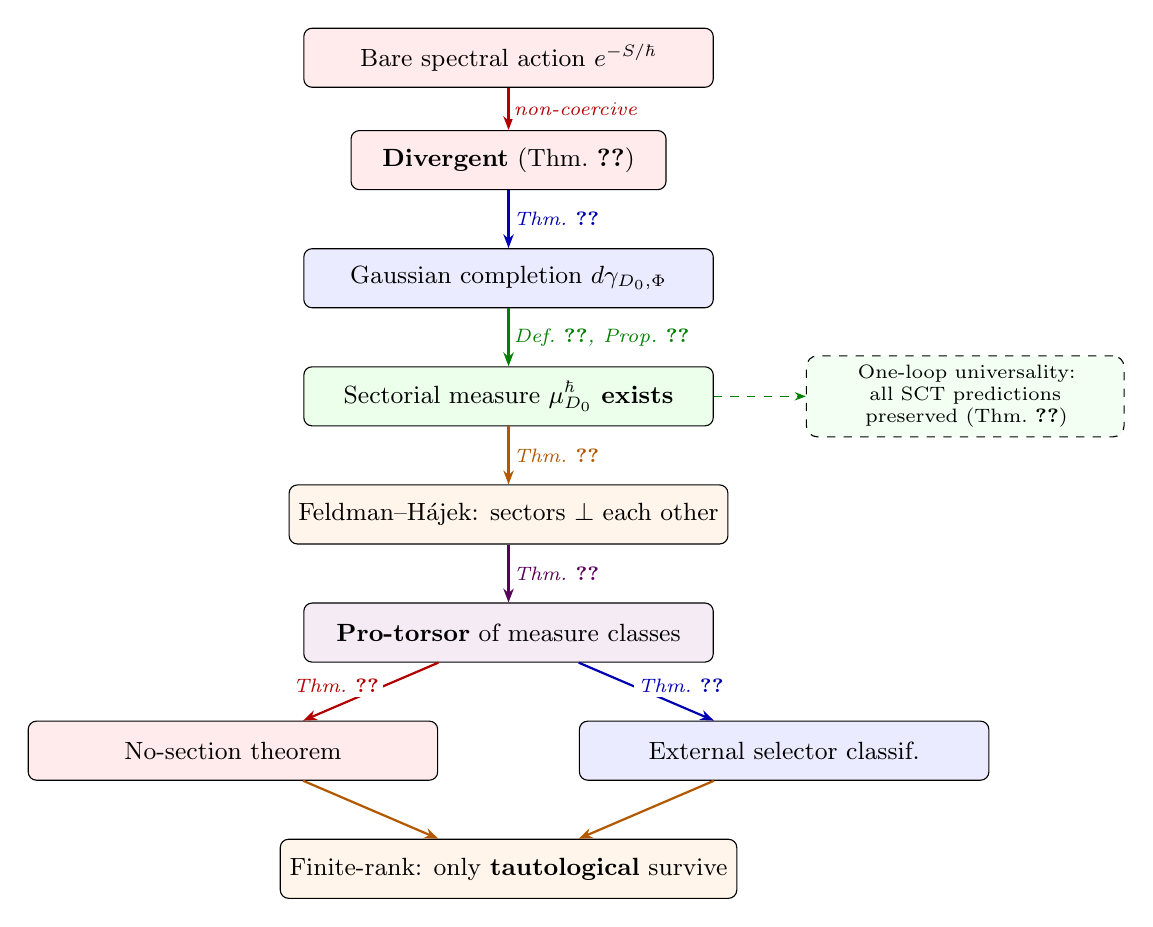
\begin{tikzpicture}[
  box/.style={draw, rounded corners=3pt, fill=#1!8, minimum width=5.2cm,
              minimum height=0.75cm, align=center, font=\small},
  box/.default=blue,
  arr/.style={-{Stealth[length=5pt]}, thick, #1},
  arr/.default=black,
  lbl/.style={font=\scriptsize\itshape, fill=white, inner sep=1.5pt},
]
% Nodes
\node[box=red]    (bare)    at (0, 0)    {Bare spectral action $e^{-S/\hbar}$};
\node[box=red,    minimum width=4cm] (div)
                            at (0,-1.3)  {\textbf{Divergent} (Thm.~\ref{thm:divergence})};
\node[box=blue]   (gauss)   at (0,-2.8)  {Gaussian completion $d\gamma_{D_0,\Phi}$};
\node[box=green]  (sect)    at (0,-4.3)  {Sectorial measure $\mu_{D_0}^\hbar$ \textbf{exists}};
\node[box=orange] (fh)      at (0,-5.8)  {Feldman--H\'ajek: sectors $\perp$ each other};
\node[box=violet] (torsor)  at (0,-7.3)  {\textbf{Pro-torsor} of measure classes};
\node[box=red]    (nosec)   at (-3.5,-8.8) {No-section theorem};
\node[box=blue]   (ext)     at (3.5,-8.8)  {External selector classif.};
\node[box=orange] (taut)    at (0,-10.3) {Finite-rank: only \textbf{tautological} survive};
% Arrows
\draw[arr=red!70!black]   (bare)   -- node[lbl,right]{non-coercive} (div);
\draw[arr=blue!70!black]  (div)    -- node[lbl,right]{Thm.~\ref{thm:sectorial-existence}} (gauss);
\draw[arr=green!50!black] (gauss)  -- node[lbl,right]{Def.~\ref{def:completed-measure}, Prop.~\ref{prop:projective}} (sect);
\draw[arr=orange!70!black](sect)   -- node[lbl,right]{Thm.~\ref{thm:feldman-hajek}} (fh);
\draw[arr=violet!70!black](fh)     -- node[lbl,right]{Thm.~\ref{thm:pro-torsor}} (torsor);
\draw[arr=red!70!black]   (torsor) -- node[lbl,left,pos=0.4]{Thm.~\ref{thm:no-section}} (nosec);
\draw[arr=blue!70!black]  (torsor) -- node[lbl,right,pos=0.4]{Thm.~\ref{thm:external-classification}} (ext);
\draw[arr=orange!70!black](nosec)  -- (taut);
\draw[arr=orange!70!black](ext)    -- (taut);
% One-loop universality note
\node[draw, dashed, rounded corners, fill=green!5,
      font=\scriptsize, text width=3.8cm, align=center]
      (univ) at (5.8,-4.3) {One-loop universality:\\all SCT predictions\\preserved (Thm.~\ref{thm:one-loop-universality})};
\draw[-{Stealth[length=4pt]}, dashed, green!50!black] (sect) -- (univ);
\end{tikzpicture}
\caption{Logical structure of the paper.  The bare spectral action
weight is non-coercive and yields a divergent integral.  A Gaussian
reference cures this sectorially, but the Feldman--H\'ajek singularity
between sectors forces a pro-torsor structure.  No internal axiom can
trivialize the torsor (principal no-section theorem); external data is
classified but constrained to tautological finite-rank channels.
All one-loop predictions are universally preserved.}
\label{fig:flow}
\end{figure}

% ============================================================
\section{The spectral action and its measure problem}
\label{sec:measure-problem}
% ============================================================

\subsection{Setup}

Let $(H, D_0, \gamma, J)$ be a compact-resolvent even real spectral
triple, where $H$ is a separable Hilbert space, $D_0$ is a self-adjoint
operator with compact resolvent $D_0 e_n = \lambda_n e_n$, $\gamma$ is
the grading, and $J$ is the real structure.  We denote the eigenvalues in
non-decreasing order of $|{\lambda_n}|$.

The self-adjoint Hilbert--Schmidt fluctuation space is
\begin{equation}\label{eq:HS-space}
  X \;:=\; \HS_\sa(H) \;=\;
  \bigl\{A \in B(H) : A = A^*,\;\Tr(A^2) < \infty\bigr\},
\end{equation}
equipped with the Hilbert--Schmidt inner product
$\langle A, B\rangle_{\HS} = \Tr(AB)$.

\begin{remark}[Choice of configuration space and gauge fixing]
\label{rem:HS-choice}
In the noncommutative-geometry framework, the physical inner
fluctuations $A = \sum a_i[D,b_i]$ are \emph{bounded} operators but
not necessarily Hilbert--Schmidt.  We work on $\HS_\sa(H)$ because
it is the largest space on which centered Gaussian probability measures
with trace-class covariance exist (see Section~\ref{sec:gaussian}).
The divergence argument of Theorem~\ref{thm:divergence} applies
\emph{a fortiori} on any subspace of $\HS_\sa(H)$, and extends to
any ambient space admitting a reference measure, since the spectral
action remains bounded by $(\dim H)\,f(0)$ on $\HS_\sa(H)$ and
converges to a finite limit along every ray.  On spaces of unbounded
operators where the spectral action may become coercive, the measure
problem takes a different form; this is beyond our scope.
We emphasize that inner fluctuations of almost-commutative spectral
triples (gauge connections, Higgs fields) are bounded operators that
are \emph{not} Hilbert--Schmidt in general: a smooth multiplication
operator on a compact manifold is bounded but not compact.
The restriction to $\HS_\sa(H)$ is therefore a genuine mathematical
choice, not a physical requirement.  Its justification is that the
Gaussian reference (Theorem~\ref{thm:sectorial-existence}) requires
trace-class covariance, which exists only on $\HS_\sa(H)$ or its
subspaces.  What is excluded
are \emph{large} fluctuations far from any background--precisely the
configurations where the one-loop approximation breaks down.
The non-perturbative measure problem for such configurations
requires different tools (e.g., lattice or CDT-type
discretization~\cite{AJL:2012}) and lies beyond the scope of this
work.

An important open question is whether the pro-torsor obstruction
(Section~\ref{sec:pro-torsor}) \emph{persists} on a larger
configuration space.  On a space where the spectral action is
coercive, the Gaussian reference may be unnecessary, and the
Feldman--H\'ajek singularity--which is driven by the product
structure of the Gaussian covariance--may not arise.  Conversely,
non-Gaussian references (e.g., Radon measures on spaces of bounded
operators) could generate a different obstruction landscape.  Until
this question is settled, the results of this paper should be
understood as applying to the \emph{Gaussian-completed
Hilbert--Schmidt framework}, not as unconditional statements about
the spectral action in general.
Furthermore, the spectral action is invariant under unitary conjugation
$D \to UDU^*$; the construction in this paper is performed on a fixed
background sector where the gauge is implicitly fixed by the choice
of~$D_0$.
The Feldman--H\'ajek singularity of
Theorem~\ref{thm:feldman-hajek} concerns the Gaussian classes
attached to different Hilbert--Schmidt background charts
$\mathcal{C}(D_0) = D_0 + \HS_\sa(H)$.
If $D_0' = UD_0U^*$ is gauge-equivalent to~$D_0$, the natural
comparison is the chart-to-chart isomorphism $J_U(A) = UAU^*$,
which is an isometry on~$X$ satisfying
$(J_U)_*\gamma_{D_0,\Phi} = \gamma_{D_0',\Phi}$ and
$(J_U)_*\mu^\hbar_{D_0} = \mu^\hbar_{D_0'}$
(because $C_{D_0',\Phi}(J_U A) = J_U(C_{D_0,\Phi}(A))$
and $S_{D_0'}(J_U A) = S_{D_0}(A)$ by trace invariance).
Thus gauge-equivalent backgrounds do \emph{not} generate a new
Feldman--H\'ajek singularity; they give isomorphic measured sectors.
The affine formula $A \mapsto UAU^* + U[D_0,U^*]$ arises only
when the transformed sector is re-expressed back in the original
chart; for almost-commutative Standard Model backgrounds the
pure-gauge term $U[D_0,U^*]$ is generically a bounded
multiplication operator but \emph{not} Hilbert--Schmidt (a
non-zero smooth multiplication operator on a compact manifold
is bounded but not compact), so this fixed-chart re-expression is
not an action on~$X$.
The Cameron--Martin obstruction of Appendix~\ref{app:cameron-martin}
applies to such \emph{fixed-chart translations} (geometric chart
shifts, which correspond to diffeomorphisms---an outer symmetry
distinct from the inner gauge group in NCG), not to the
chart-to-chart identification $J_U$.
Accordingly, Theorem~\ref{thm:feldman-hajek} should be interpreted
as an obstruction between gauge-\emph{inequivalent} background
sectors (distinct spectra = distinct gauge orbits), while a fully
global quotient-level construction still requires an explicit
gauge-fixed atlas and Faddeev--Popov analysis; see
Section~\ref{sec:not-shown}.
\end{remark}

For a fixed background $D_0$, the total Dirac operator is
$D = D_0 + A$ with $A \in X$.  The spectral action evaluated on
the fluctuation is
\begin{equation}\label{eq:SA-fluctuation}
  S(A) \;:=\; \Tr\, f\!\left(\frac{(D_0+A)^2}{\Lam^2}\right),
\end{equation}
where $f\colon [0,\infty) \to [0,\infty)$ is a positive even
Schwartz-class function.

\subsection{Divergence of the naive integral}

The positivity and boundedness of $f$ immediately constrain $S$:

\begin{lemma}\label{lem:bounded}
For every $A \in X$, $S(A) \ge 0$.  On any finite-rank
slice $\Omega_N$ of dimension $d_N$,
\begin{equation}
  0 \;\le\; S_N(A) \;\le\; d_N\,f(0).
\end{equation}
In infinite dimensions ($\dim H = \infty$), the full spectral action
$S(A) = \sum_j f(\mu_j^2/\Lam^2)$ is finite for every $A$ (since $f$
is Schwartz and $D_0 + A$ has Weyl-growing eigenvalues), but
$S(A) \le S(0) := \sum_j f(\lambda_j^2/\Lam^2) < \infty$ does
\emph{not} hold in general.
\end{lemma}

\begin{proof}
Since $f \ge 0$, every summand $f(\mu_j^2/\Lam^2) \ge 0$, giving
$S \ge 0$.  On $\Omega_N$, there are $d_N$ eigenvalues, each
contributing at most $f(0)$.
\end{proof}

\begin{theorem}[Divergence of the naive integral]
\label{thm:divergence}
Let $V \subset X$ be any nonzero finite-dimensional subspace.  Then
\begin{equation}
  \int_V \exp\!\bigl(-S(A)/\hbar\bigr)\,\dd A \;=\; +\infty.
\end{equation}
\end{theorem}

\begin{proof}
It suffices to show that $\exp(-S(A)/\hbar)$ is bounded below by a
positive constant along every ray in~$V$, since $V$ contains
unbounded rays and the resulting lower-bounded integral over each
ray diverges.

Fix any nonzero $A_1 \in V$ and consider the ray $A(t) = tA_1$,
$t \in \R$.  The operator $D(t) := D_0 + tA_1$ has eigenvalues
$\mu_n(t)$.  Since $A_1 \in \HS_\sa(H)$ is compact,
Weyl's inequality gives $|\mu_n(t) - \lambda_n| \le t\,\|A_1\|$,
so $|\mu_n(t)| \ge |\lambda_n| - |t|\,\|A_1\|$.  For each
fixed~$t$, the spectral tail satisfies $|\mu_n(t)| \to \infty$ as
$n \to \infty$, hence $f(\mu_n(t)^2/\Lam^2) \to 0$ along the tail
(since $f \ge 0$ and $f(u) \to 0$ as $u \to \infty$).

The action $S(tA_1) = \sum_n f(\mu_n(t)^2/\Lam^2)$ is therefore a
convergent sum of non-negative terms, each bounded by~$f(0)$.  As
$|t| \to \infty$, the eigenvalues of $D(t)$ are pushed away from
the origin: for any fixed~$R > 0$, only finitely many indices~$n$
satisfy $|\mu_n(t)| \le R$ when $|t|$ is large (since $|\lambda_n|$
grows and $A_1$ is compact).  Therefore the number of terms
contributing more than~$\delta$ to the sum tends to zero, and
$S(tA_1) \to c_{A_1}$ for some finite $c_{A_1} \ge 0$.

Hence $\exp(-S(tA_1)/\hbar) \to \exp(-c_{A_1}/\hbar) > 0$, and the
integral along the ray $\int_{-\infty}^\infty \exp(-S(tA_1)/\hbar)\,
\dd t = +\infty$ (by comparison with a positive constant on an
unbounded interval).  Since $V$ contains such a ray, the
$d$-dimensional integral over~$V$ diverges.
\end{proof}

\begin{remark}
Theorem~\ref{thm:divergence} shows that neither a global minimum
principle nor a naive path integral is available for the spectral
action.  The weight $\exp(-S/\hbar)$ is essentially constant at
infinity, and the configuration space is non-compact.
A \emph{completion} of the exponent--by a reference measure, a
coercive term, or a domain restriction--is mandatory.
\end{remark}

\subsection{Smooth-window truncations and convergence}
\label{subsec:smooth-window}

For a smooth compactly supported cutoff $\chi_R \in C_c^\infty(\R)$
with $0 \le \chi_R \le 1$, $\chi_R(\lambda) = 1$ for
$|\lambda| \le R$, and $\mathrm{supp}\,\chi_R \subset
\{|\lambda| \le R+1\}$, define the smooth-window truncated action
\begin{equation}\label{eq:smooth-window}
  S_R(A) \;:=\; \Tr\bigl(\chi_R(D_0+A)\,f((D_0+A)^2/\Lam^2)\bigr).
\end{equation}
Since $\chi_R(D_0+A)$ is a spectral function of $D_0+A$, it commutes
with all bounded Borel functions of $D_0+A$, eliminating the
projection/compression mismatch that afflicts frozen-projector
truncations.

\begin{theorem}[Smooth-window convergence]
\label{thm:smooth-convergence}
Assume the following standard spectral-perturbation hypotheses:
\begin{enumerate}[label=\textup{(A\arabic*)},leftmargin=3em]
  \item\label{A1} All operators $D(A) := D_0 + A$ share a common
    dense domain $\mathrm{Dom}(D_0) \subset H$.
  \item\label{A2} The parameter derivatives $\partial_i D$ and
    $\partial_{ij} D$ are first-order differential operators with
    uniformly bounded matrix elements:
    $|\langle e_m, \partial_i D\, e_n\rangle| \le C(1+|\lambda_m|)^{1/2}
    (1+|\lambda_n|)^{1/2}$.
  \item\label{A3} Uniform Weyl counting:
    $N_A(L) := \#\{n : |\mu_n(A)| \le L\} \le C_K(1+L)^d$ on compact
    parameter subsets $K$.
  \item\label{A4} Schwartz divided differences: the first and second
    divided differences of any Schwartz function are again Schwartz on
    $\R^2$ and $\R^3$, respectively.
\end{enumerate}
Then for every compact parameter subset $K$,
\begin{equation}
  \sup_{A \in K}\,\bigl|\partial_A^\alpha\bigl(S_R(A) - S(A)\bigr)\bigr|
  \;\longrightarrow\; 0
  \qquad\text{as } R \to \infty,
  \quad |\alpha| \le 2.
\end{equation}
If\, $f$ has Schwartz decay $|f^{(k)}(\lambda)| \le C_k
(1+|\lambda|)^{-M}$ for all $M$, the convergence rate is
\begin{equation}\label{eq:convergence-rate}
  \bigl|S_R(A) - S(A)\bigr| \;\le\; C_K\,(1+R)^{d-M}
\end{equation}
for any $M > 0$, with analogous estimates for derivatives.  For
exponentially decaying $f(\lambda) \sim e^{-c\lambda}$, the rate is
$\order(e^{-cR})$.
\end{theorem}

\begin{proof}[Proof sketch]
Write $r_R := (1-\chi_R)\cdot h$ where $h(\lambda) :=
f(\lambda^2/\Lam^2)$.  Since $\chi_R = 1$ for $|\lambda| \le R$ and
$h$ is Schwartz, $r_R \to 0$ in the Schwartz topology.  The first
derivative of the spectral action uses the Hellmann--Feynman formula
(multiple operator integral of order 1), and the second derivative
uses the double sum over divided differences.  Under
\ref{A1}--\ref{A4}, the matrix element bounds and Weyl counting
ensure uniform convergence of these sums.  The rate
estimate~\eqref{eq:convergence-rate} follows from the tail bound
$|r_R(\lambda)| \le C(1+R)^{-M}$ for $|\lambda| > R$.  Full
details are in Appendix~\ref{app:convergence}.
\end{proof}

\begin{corollary}[Saddle persistence]
\label{cor:saddle-persistence}
If $A_* = 0$ is a nondegenerate critical point of $S$ on a gauge-fixed
slice, then for all sufficiently large $R$, $S_R$ has a unique nearby
critical point $A_R \to A_*$ with converging Hessian.
\end{corollary}

% ============================================================
\section{Corrected functional Gaussian and sectorial existence}
\label{sec:gaussian}
% ============================================================

The divergence theorem motivates introducing an ambient reference
measure that supplies the missing coercivity.  We work with centered
Gaussian measures on the operator space~$X$.

\subsection{Two-sided functional Gaussian covariance}

\begin{definition}\label{def:covariance}
Let $\Phi\colon [0,\infty) \to (0,\infty)$ be a positive admissible
spectral weight (e.g., heat-kernel $\Phi(u) = e^{-u}$ or Sobolev
$\Phi(u) = (1+u)^{-s}$, $s > 2$).  Define the spectral decay
coefficients $\phi_n := \Phi(\lambda_n^2/\Lam^2)$ and the two-sided
covariance operator
\begin{equation}\label{eq:covariance}
  C_\Phi(A) \;:=\; \sigma^2\, \Phi_0\, A\, \Phi_0,
  \qquad \Phi_0 := \Phi(D_0^2/\Lam^2),
\end{equation}
acting on $X = \HS_\sa(H)$, where $\sigma^2 > 0$ is a
normalization constant.
\end{definition}

In the eigenbasis $\{E_{mn}\}$ of $D_0$, the covariance acts
diagonally on matrix units:
$C_\Phi(E_{mn}) = \sigma^2 \phi_m \phi_n\, E_{mn}$.

\begin{theorem}[Trace-class criterion]
\label{thm:trace-class}
The operator $C_\Phi$ is trace-class on $X = \HS_\sa(H)$ if and only if
\begin{equation}\label{eq:trace-class-condition}
  \sum_{n=0}^\infty \phi_n \;<\; \infty.
\end{equation}
When this holds, $\Tr_{\HS}(C_\Phi) = \sigma^2\bigl(\sum_n
\phi_n\bigr)^2$.
\end{theorem}

\begin{proof}
Choose the real orthonormal basis of $\HS_\sa(H)$ consisting of the
diagonal matrix units $F_{nn} := E_{nn}$ and the off-diagonal units
$(E_{mn} + E_{nm})/\sqrt{2}$ and $i(E_{mn} - E_{nm})/\sqrt{2}$ for
$m < n$.  Then $C_\Phi(F_{nn}) = \sigma^2 \phi_n^2 F_{nn}$,
contributing $\sigma^2\phi_n^2$ to the trace.  Each off-diagonal pair
contributes $\sigma^2 \phi_m\phi_n$.  Summing:
$\Tr_{\HS}(C_\Phi) = \sigma^2[\sum_n \phi_n^2 + 2\sum_{m<n}
\phi_m\phi_n] = \sigma^2(\sum_n \phi_n)^2$.  This is finite iff
$\sum_n \phi_n < \infty$.
\end{proof}

\begin{proposition}[Admissibility of standard spectral weights]
\label{prop:admissibility}
\hfill
\begin{enumerate}[label=\textup{(\alph*)},leftmargin=2.5em]
  \item Heat-kernel: $\Phi(u) = e^{-\tau u}$, $\tau > 0$.  Then
    $\phi_n = e^{-\tau\lambda_n^2/\Lam^2}$, and $\sum_n \phi_n <
    \infty$ by Weyl asymptotics $|\lambda_n| \sim n^{1/d}$.
  \item Sobolev: $\Phi(u) = (1+u)^{-s}$, $s > 0$.  Then $\sum_n
    \phi_n < \infty$ iff $s > d/2$.  For $d=4$, this requires $s > 2$.
  \item SCT one-loop kernels: $\Phi(u) \sim c/u$ as $u \to \infty$.
    Then $\phi_n \sim c\Lam^2/\lambda_n^2$, giving $\sum_n \phi_n
    \sim \sum_n n^{-2/d}$, which diverges for $d \ge 2$.
    \textbf{The SCT master function and one-loop form factors do not
    define admissible covariances.}
\end{enumerate}
\end{proposition}

\begin{remark}[SCT one-loop kernels versus the reference measure]
\label{rem:kernels-vs-reference}
The non-admissibility of the SCT one-loop kernels as Gaussian
covariances does \emph{not} undermine the one-loop universality
theorem (Theorem~\ref{thm:one-loop-universality}).  The distinction
is between the \emph{input} and the \emph{output} of the construction:
the spectral weight $\Phi$ is the \emph{input} that defines the
reference measure, while the SCT form factors $h_C, h_R$ are the
\emph{output} of the one-loop perturbative computation around any
admissible reference.  Theorem~\ref{thm:one-loop-universality}
states that this output is the same for every admissible $\Phi$,
and equals the standard stationary-phase result.  The SCT form factors
thus characterize the universal one-loop effective action, not the
reference covariance.
\end{remark}

\subsection{Sectorial existence theorem}

\begin{theorem}[Sectorial Gaussian parent measure]
\label{thm:sectorial-existence}
For every fixed compact-resolvent background $D_0$ and every admissible
weight $\Phi$ with $\sum_n \phi_n < \infty$, there exists a unique
centered Gaussian Borel probability measure
\begin{equation}
  \gamma_{D_0,\Phi}
\end{equation}
on $X = \HS_\sa(H)$ with covariance $C_\Phi$.
\end{theorem}

\begin{proof}
Since $C_\Phi$ is a symmetric positive trace-class operator on the
separable Hilbert space $X$, the existence and uniqueness of
$\gamma_{D_0,\Phi}$ follow from the standard theory of Gaussian
measures on separable Hilbert spaces
(see \cite{Bogachev:1998}, Chapter~3; \cite{Kuo:1975}).  Alternatively,
the measure is the product of one-dimensional Gaussians
$\mathcal{N}(0, \sigma^2\phi_m\phi_n)$ in the eigenbasis, and the
product converges by Kolmogorov's consistency theorem since the
product of variances $\prod_{m,n}(1 + \sigma^2\phi_m\phi_n)$ converges
when $\sum_{m,n}\phi_m\phi_n = (\sum_n \phi_n)^2 < \infty$.
\end{proof}

\begin{definition}[Sectorial completed measure]
\label{def:completed-measure}
The \emph{sectorial completed measure} for background $D_0$, spectral
weight $\Phi$, and loop-expansion parameter $\hbar > 0$
(introduced as a formal saddle-point control; the spectral action
$S$ itself is $\hbar$-independent, and $\hbar$ enters only through
the weight $\exp(-S/\hbar)$, playing the same role as in the
standard loop expansion of quantum field theory) is
\begin{equation}\label{eq:completed-measure}
  \dd\mu_{D_0}^\hbar(A)
  \;:=\;
  \frac{1}{Z_{D_0}}\,
  \exp\!\left(-\frac{S(A)}{\hbar}\right)
  \dd\gamma_{D_0,\Phi}(A),
\end{equation}
where $Z_{D_0} := \int_X \exp(-S(A)/\hbar)\,\dd\gamma_{D_0,\Phi}(A)$.
\end{definition}

\begin{proposition}[Finite partition function]
\label{prop:finite-Z}
$0 < Z_{D_0} \le 1$.  Hence $\mu_{D_0}^\hbar$ is a well-defined
probability measure on~$X$, absolutely continuous with respect to
$\gamma_{D_0,\Phi}$.
\end{proposition}

\begin{proof}
Since $S(A) \ge 0$ for all $A$, the integrand satisfies
$0 < \exp(-S/\hbar) \le 1$.  Hence $0 < Z_{D_0} \le
\gamma_{D_0,\Phi}(X) = 1$.
\end{proof}

\subsection{Projective compatibility}

Let $P_N$ denote the spectral projection of $|D_0|$ onto its first
$N+1$ eigenvalues, and define the truncation map
$\pi_N(A) := P_N A P_N$.  Write
$\mu_{D_0,N}^\hbar := (\pi_N)_*\mu_{D_0}^\hbar$ for the pushforward
to the finite-dimensional space $\Omega_N := P_N X P_N$.

\begin{proposition}[Exact projective compatibility]
\label{prop:projective}
For every $M \ge N$,
$(\pi_{M \to N})_*\,\mu_{D_0,M}^\hbar = \mu_{D_0,N}^\hbar$,
where $\pi_{M \to N}$ is the natural projection from $\Omega_M$ to
$\Omega_N$.
\end{proposition}

\begin{proof}
The covariance $C_\Phi$ is diagonal in the eigenbasis, so the
Gaussian reference $\gamma_{D_0,\Phi}$ is a product measure.
Truncation $\pi_N$ projects onto a coordinate subspace, and
pushforward of a product Gaussian onto a coordinate subspace is
the corresponding marginal Gaussian.  Since the spectral action
$S(A)$ depends on \emph{all} eigenvalues of $D_0 + A$, the
completed measure is not a product.  However, the exact
projective compatibility follows from the standard disintegration:
for test function $\varphi$ on $\Omega_N$,
\begin{align*}
  \int_{\Omega_N}\varphi\,\dd\mu_{D_0,N}^\hbar
  &= \int_X (\varphi \circ \pi_N)\,\dd\mu_{D_0}^\hbar
  = \frac{1}{Z}\int_X (\varphi\circ\pi_N)\,e^{-S/\hbar}\,\dd\gamma \\
  &= \frac{1}{Z}\int_{\Omega_M}
    \left(\int_{\pi_{M\to N}^{-1}(x)}
      (\varphi\circ\pi_{M\to N})(y)\,e^{-S(y)/\hbar}
    \,\dd\gamma^x(y)\right)\dd\gamma_M(x),
\end{align*}
which yields the same answer whether we first push down to $\Omega_M$
and then to $\Omega_N$, or directly to $\Omega_N$.
\end{proof}

\subsection{One-loop universality}
\label{subsec:one-loop}

\begin{theorem}[One-loop universality of expectations]
\label{thm:one-loop-universality}
Let $\Phi$ and $\Psi$ be two admissible spectral weights, both with
$\sum_n \phi_n < \infty$ and $\sum_n \psi_n < \infty$.
Suppose that the background $A_* = 0$ is a nondegenerate critical
point of the physical-slice action $S_N$ (i.e.\ $H_{*,N} :=
\nabla^2 S_N(0)$ is positive-definite on~$\Omega_N$).
Then for any $O \in C^3_b(\Omega_N)$,
\begin{equation}\label{eq:one-loop-univ}
  \langle O \rangle_\Phi
  \;=\; O(0)
  + \frac{\hbar}{2}\sum_i \frac{\partial^2 O}{\partial \xi_i^2}(0)\,
    (H_*^{-1})_{ii}
  + \order(\hbar^2)
  \;=\; \langle O \rangle_\Psi,
\end{equation}
where $\xi_i$ denote the principal-axis coordinates on $\Omega_N$
diagonalizing $H_{*,N}$, and
$H_* = \nabla^2 S(0)|_{\mathrm{phys}}$ is the physical-slice
Hessian at the background.  The reference measure $\Phi$ enters
expectation values only at order $\order(\hbar^2)$.
\end{theorem}

\begin{proof}
Since $O$ depends only on the finite-rank projection
$\pi_N(A) \in \Omega_N$, we work on $\Omega_N$ (dimension $d_N$)
throughout; the integral over complementary (high) modes
factorizes identically in numerator and denominator of
$\langle O\rangle_\Phi = N/Z$ and cancels in the ratio.

On the \emph{finite-dimensional} slice $\Omega_N$, write the
completed measure as
$\dd\mu_N^\hbar(x) \propto \exp\bigl(-S_N(x)/\hbar
- x^T C_{\Phi,N}^{-1} x/2\bigr)\,\dd x$,
where $S_N$ is the truncated action and $C_{\Phi,N}$ is the
$d_N \times d_N$ marginal covariance.  The effective precision
on $\Omega_N$ is
\[
  Q_{\hbar,N} \;=\; \frac{H_{*,N}}{\hbar} + C_{\Phi,N}^{-1},
\]
where $H_{*,N} = \nabla^2 S_N(0)$.  Since $\Omega_N$ is
finite-dimensional, both $H_{*,N}$ and $C_{\Phi,N}^{-1}$ are
$d_N \times d_N$ matrices, and the Neumann series
\[
  Q_{\hbar,N}^{-1}
  = \hbar\,H_{*,N}^{-1}
  - \hbar^2\,H_{*,N}^{-1}C_{\Phi,N}^{-1}H_{*,N}^{-1}
  + \order(\hbar^3)
\]
converges for sufficiently small $\hbar$ (specifically, for
$\hbar < \|H_{*,N}^{-1}\|^{-1}\|C_{\Phi,N}^{-1}\|^{-1}$, which is
positive since both matrices are finite-dimensional and
positive-definite).  The leading covariance
$\hbar\,H_{*,N}^{-1}$ is independent of~$\Phi$.

The standard finite-dimensional Laplace formula for the ratio
$\langle O\rangle = N/Z$ then gives
\[
  \langle O\rangle_\Phi
  = O(0) + \frac{\hbar}{2}\,\Tr\bigl(O''(0)\,H_{*,N}^{-1}\bigr)
  + \order(\hbar^2),
\]
which depends only on the physical Hessian $H_{*,N}$, not
on~$C_{\Phi,N}$.  The $\Phi$-dependent correction enters at
$\order(\hbar^2)$ through the subleading term
$\hbar^2 H_{*,N}^{-1}C_{\Phi,N}^{-1}H_{*,N}^{-1}$.

\emph{Factorization of high modes.}
Let $\Omega_N^\perp$ denote the complementary spectral subspace.
In the spectral eigenbasis of~$D_0$, the physical Hessian
$H_* = \nabla^2 S(0)$ acts diagonally on the matrix units
$E_{mn}$, so the cross-block $H_{*,\mathrm{low\text{-}high}} = 0$
at quadratic order.
Write $S(x,y) = S_N(x) + S_\perp(y) + S_{\mathrm{mix}}(x,y)$
where $S_{\mathrm{mix}} = O(|x|\,|y|^2) + O(|x|^2\,|y|)$ starts at
cubic order.  The Gaussian reference $\gamma_\Phi$ has product
structure: $\gamma_\Phi = \gamma_{\Phi,N}\otimes\gamma_{\Phi,\perp}$.
Therefore the marginal of
$e^{-S/\hbar}\,d\gamma_\Phi$ on $\Omega_N$ is
\[
  \Bigl[\int_{\Omega_N^\perp} e^{-S_\perp(y)/\hbar
  - S_{\mathrm{mix}}(x,y)/\hbar}\,
  \dd\gamma_{\Phi,\perp}(y)\Bigr]\,
  e^{-S_N(x)/\hbar}\,\dd\gamma_{\Phi,N}(x).
\]
At quadratic order ($\hbar \to 0$), $S_{\mathrm{mix}}$ is subleading,
the bracket becomes $x$-independent, and cancels in the ratio
$\langle O\rangle = N/Z$
for any~$O$ supported on~$\Omega_N$.
The $\Phi$-dependence of the bracket is likewise a common
factor in~$N$ and~$Z$; its first $x$-dependent correction enters at
$O(\hbar^2)$ through the cubic vertices of~$S$.
\end{proof}

\begin{remark}[Scope of universality: expectations vs.\ partition
function]
\label{rem:univ-scope}
Theorem~\ref{thm:one-loop-universality} establishes
$\Phi$-independence for \emph{normalized expectations}
$\langle O\rangle = N/Z$, where the $\Phi$-dependent factors cancel in
the ratio.  The \emph{partition function}~$Z$ itself is
$\Phi$-dependent even at leading order (through normalization constants
of $\gamma_\Phi$).  The \emph{one-loop effective action}
$\Gamma^{(1)} = \half\Tr\log H_*$ in the SCT literature is defined via
$\zeta$-function regularization of the physical Hessian $H_*$
(see~\cite{Alfyorov:2026ff}), which is an intrinsic spectral invariant
of $H_*$ and independent of $\Phi$ by construction.  Any one-loop
quantity extractable from $\Gamma^{(1)}$ (form factors, spectral
coefficients, propagator poles) is therefore $\Phi$-independent.
See Appendix~\ref{app:alpha} for specific numerical values.
\end{remark}

\begin{remark}[Status beyond one loop]
\label{rem:beyond-one-loop}
The $\order(\hbar^2)$ dependence on $\Phi$ means that two-loop and
higher corrections are \emph{not} universal: they carry an imprint of
the reference measure.  This has three possible interpretations:
(i)~the spectral action is an effective theory valid only at one loop,
with the reference-measure ambiguity absorbing unknown UV physics;
(ii)~a physical principle (yet to be identified) selects a preferred
$\Phi$, restoring predictivity at two loops;
(iii)~the density-valued formalism of the pro-torsor is the
correct framework, and two-loop ``predictions'' should be stated as
sections of the density line rather than as scalar numbers.
This paper does not resolve the choice among (i)--(iii); it merely
establishes the framework in which the question is precisely posed.
We note that interpretation~(i) is the spectral-geometric analogue of
a well-established situation: general relativity, viewed as an
effective field theory~\cite{Donoghue:1994}, is predictive at one loop
but acquires scheme-dependent corrections at two loops that parametrize
unknown UV physics.  The $\Phi$-dependence at $\order(\hbar^2)$ plays
the same role as the renormalization-scheme dependence in gravitational
EFT, and is no more pathological.
We note that the analogy with scheme dependence is heuristic: in
standard EFT, physical observables remain scheme-independent at any
finite loop order when all counterterms are included, whereas the
reference-measure dependence here reflects an incomplete
non-perturbative definition rather than a conventional
renormalization ambiguity.
\end{remark}

\begin{remark}\label{rem:universality-consequence}
Theorem~\ref{thm:one-loop-universality} is physically essential: it
guarantees that the one-loop spectral causal theory results
reported in~\cite{Alfyorov:2026ff,Alfyorov:2026ss,Alfyorov:2026ct}--the
Weyl-squared coefficient $\alpha_C =
13/120$~\cite{Alfyorov:2026ff}, the ghost pole and fakeon
mass~\cite{AlfyorovShnyukov:2026ns}, and the parametrized
post-Newtonian bounds~\cite{Alfyorov:2026ss}--are
\emph{independent} of the choice of Gaussian reference.
(We note that references~\cite{Alfyorov:2026ff,Alfyorov:2026ss,%
AlfyorovShnyukov:2026ns} are preprints currently under peer review;
the one-loop results cited are self-contained and independently
verifiable from the derivations therein.)
\end{remark}

\subsection{Concrete example: the two-mode matrix model}
\label{subsec:example}

To make the construction explicit, consider the simplest nontrivial
case: a two-dimensional Hilbert space $H = \mathbb{C}^2$ with
background $D_0 = \mathrm{diag}(\lambda_1, \lambda_2)$,
$\lambda_1 \ne \lambda_2$.  The spectral action is
\begin{equation}
  S(A) = f\!\left(\frac{(\lambda_1+a_{11})^2}{\Lam^2}\right)
       + f\!\left(\frac{(\lambda_2+a_{22})^2}{\Lam^2}\right)
\end{equation}
where we restrict to diagonal fluctuations
$A = \mathrm{diag}(a_{11}, a_{22})$ for simplicity (off-diagonal
entries mix eigenvalues nonlinearly but do not affect the divergence
argument).

\begin{example}[Two-mode completed integral]
\label{ex:two-mode}
The bare integral $\int_{\R^2} e^{-S(a)/\hbar}\,\dd a$ diverges by
Theorem~\ref{thm:divergence}: along $a_{11} \to \infty$ with
$a_{22} = 0$, $S \to f(\lambda_2^2/\Lam^2) > 0$ constant, so the
integrand is bounded below.

With Gaussian reference $\dd\gamma(a) \propto
\exp(-a_{11}^2/(2\sigma^2\phi_1^2) - a_{22}^2/(2\sigma^2\phi_2^2))\,
\dd a$, the completed integral is
\begin{equation}
  Z = \int_{\R^2} e^{-S(a)/\hbar}\,\dd\gamma(a)
  \;\le\; 1,
\end{equation}
which is finite and positive.  The one-loop approximation gives
$Z \approx e^{-S_*/\hbar}\,(2\pi\hbar)/(H_{11}H_{22})^{1/2}$,
independent of $\sigma$ and $\phi_j$.

Now consider a second background $D_0' = \mathrm{diag}(\lambda_1',
\lambda_2')$ with $\lambda_j' \ne \lambda_j$.  The Gaussian
references $\gamma$ and $\gamma'$ have different
covariances ($\phi_j \ne \phi_j'$), but in two dimensions both are
non-degenerate Gaussians on $\R^2$, hence \emph{equivalent} (not
singular).  This illustrates two key points: (1)~the Gaussian completion cures the
divergence at any rank; (2)~at \emph{finite rank}, the Feldman--H\'ajek
singularity does not arise--different backgrounds give equivalent (not
singular) measures.  The pro-torsor structure is a genuinely
infinite-dimensional phenomenon
(Section~\ref{sec:pro-torsor}).
\end{example}

\begin{figure}[ht]
\centering
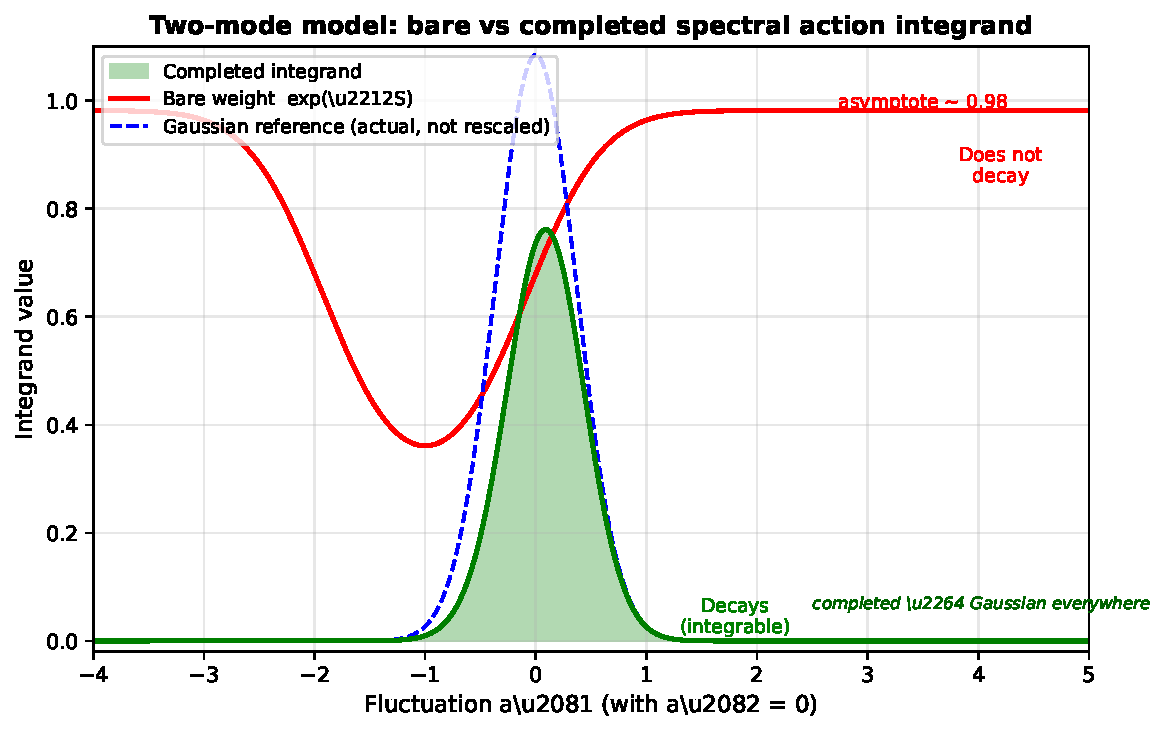
\includegraphics[width=0.82\textwidth]{fig_nonpert_2mode.pdf}
\caption{Two-mode matrix model ($H = \mathbb{C}^2$,
$D_0 = \mathrm{diag}(1,2)$, $f(u) = e^{-u}$, $\Lam = 1$).
Red: the bare integrand $e^{-S(a_1,0)/\hbar}$ does not decay as
$|a_1| \to \infty$ (approaches $e^{-f(\lambda_2^2)} \approx 0.98$),
making the naive integral divergent
(Theorem~\ref{thm:divergence}).
Green: the completed integrand, reweighted by the Gaussian reference
$d\gamma$ with covariance $\sigma^2\phi_1^2 \approx 0.135$
($\hbar = \sigma = 1$), decays rapidly and yields a finite partition
function $Z \approx 0.67$.
Blue dashed: Gaussian reference density (actual, not rescaled).
Since $S \ge 0$, the completed integrand is bounded above by the
Gaussian density everywhere: $e^{-S}\,d\gamma \le d\gamma$.
Integrals computed using \texttt{mpmath} quadrature at 100-digit
working precision with absolute tolerance~$10^{-50}$.}
\label{fig:2mode}
\end{figure}

% ============================================================
\section{Pro-torsor structure and density-valued observables}
\label{sec:pro-torsor}
% ============================================================

We now turn to the global structure that emerges when different
background sectors are assembled.

\subsection{Feldman--H\'ajek singularity}

\begin{theorem}[Feldman--H\'ajek rigidity for spectral covariances]
\label{thm:feldman-hajek}
Let $D_0$ and $D_0'$ be two compact-resolvent backgrounds
\emph{sharing a common eigenbasis}, with eigenvalues
$\{\lambda_n\}$ and $\{\lambda_n'\}$, and let $\gamma_{D_0,\Phi}$
and $\gamma_{D_0',\Phi}$ be the corresponding centered Gaussian
measures on $X = \HS_\sa(H)$ with the same spectral weight~$\Phi$.
Then $\gamma_{D_0,\Phi} \perp \gamma_{D_0',\Phi}$ unless
$\phi_n = \phi_n'$ for all~$n$.  In particular, any nontrivial
change of the background eigenvalues (within a fixed eigenbasis)
produces a mutually singular Gaussian reference.
\end{theorem}

\begin{proof}
By the Feldman--H\'ajek
theorem~\cite{Feldman:1958,Hajek:1958,Bogachev:1998}, two centered
Gaussian measures on a separable Hilbert space are either equivalent or
mutually singular; they are equivalent iff
$C_\Phi^{-1/2} C_{\Phi'} C_\Phi^{-1/2} - I$ is Hilbert--Schmidt.

In the eigenbasis of~$D_0$
(the general case follows from the abstract criterion),
the eigenvalues of
$C_\Phi^{-1/2} C_{\Phi'} C_\Phi^{-1/2}$ on the matrix unit $E_{mn}$
are $r_m r_n$, where $r_n := \phi_n'/\phi_n$.  The HS condition
becomes $\sum_{m,n}(r_m r_n - 1)^2 < \infty$.  Setting
$s_k := r_k - 1$:
\[
  r_m r_n - 1 = s_m + s_n + s_m s_n.
\]
For any fixed $m$ with $s_m \ne 0$, we show the sum over~$n$
diverges.  Two cases arise.

\emph{Case~1: $r_n \to 1$ (i.e.\ $s_n \to 0$).}  This occurs when
the eigenvalue perturbation is small enough that $\phi_n'/\phi_n \to 1$
along the spectral tail.  Then for all sufficiently large~$n$,
$|s_n| < |s_m|/2$, and $(r_m r_n - 1)^2 = (s_m(1+s_n)+s_n)^2
\ge (|s_m|/2)^2 = s_m^2/4 > 0$.

\emph{Case~2: $r_n \not\to 1$.}  If $r_n \to c \ne 1$ (including
$c = 0$ or $c = +\infty$, which occur when $\lambda_n' - \lambda_n$
grows), then $r_m r_n - 1 \to r_m c - 1 \ne 0$ for infinitely many
$n$, and each such term contributes a positive constant.

In both cases the tail of the sum over~$n$ contains infinitely many
terms bounded below by a positive constant, giving
\[
  \sum_{n=0}^\infty (r_m r_n - 1)^2 \;=\; +\infty.
\]
Therefore the double sum is finite only if $s_m = 0$ for \emph{every}
$m$, i.e., $r_m = 1$ and $\phi_m = \phi_m'$ for all~$m$.
\end{proof}

\begin{remark}[General backgrounds]
\label{rem:fh-general}
Theorem~\ref{thm:feldman-hajek} is stated for backgrounds sharing a
common eigenbasis.  When $D_0$ and $D_0'$ have distinct eigenbases,
the covariance operators $C_\Phi$ and $C_{\Phi'}$ do not
simultaneously diagonalize, and the Feldman--H\'ajek criterion
involves the full operator
$C_\Phi^{-1/2}C_{\Phi'}C_\Phi^{-1/2} - I$ rather than a product
of scalar ratios.  We conjecture that singularity persists in this
case as well, since any $\varepsilon$-perturbation of the spectrum
changes the spectral weight values $\phi_n$; a complete proof
requires verifying the Hilbert--Schmidt condition for the
non-diagonal operator and is left for future work.
\end{remark}

\begin{proposition}[Universal singularity for perturbatively close
backgrounds]
\label{prop:fh-close}
Let $D_0$ and $D_0'$ be two compact-resolvent backgrounds
\emph{sharing a common eigenbasis}, with
$\phi_k \ne \phi_k'$ for at least one index~$k$.  Then
$\gamma_{D_0,\Phi} \perp \gamma_{D_0',\Phi}$.
In particular, if $D_0' = D_0 + \varepsilon K$ with $\varepsilon > 0$
and $K$ any nonzero self-adjoint perturbation that changes at least one
eigenvalue of~$D_0$, then the measures are mutually singular--even for
arbitrarily small $\varepsilon$ and even for finite-rank~$K$.
\end{proposition}

\begin{proof}
If $\phi_k \ne \phi_k'$, set $s_k = r_k - 1 \ne 0$.  Then
$\sum_n (r_k r_n - 1)^2 \ge \sum_n s_k^2 = +\infty$
(infinitely many terms), so the Feldman--H\'ajek sum diverges and
Theorem~\ref{thm:feldman-hajek} gives singularity.
\end{proof}

\begin{remark}\label{rem:fh-sharpness}
The strength of Proposition~\ref{prop:fh-close} deserves emphasis.
Unlike standard Gaussian measure theory on $\ell^2$ (where changing a
single coordinate variance preserves equivalence), the \emph{product
structure} of the spectral covariance
$C_\Phi(E_{mn}) = \sigma^2\phi_m\phi_n$ means that altering a single
spectral decay coefficient $\phi_k$ changes the covariance eigenvalue
for \emph{every} matrix unit $E_{kn}$, $n = 0,1,2,\ldots$--infinitely
many eigenvalues.  This is why even a rank-$1$ perturbation of $D_0$
produces mutual singularity on the infinite-dimensional space
$\HS_\sa(H)$.

At \emph{finite} spectral rank $N$ (Example~\ref{ex:two-mode}), the
configuration space $\Omega_N$ is finite-dimensional and all
nondegenerate Gaussians are equivalent--the Feldman--H\'ajek dichotomy
does not apply.  The singularity is a genuinely infinite-dimensional
phenomenon arising from the product structure of operator-space
Gaussians.
\end{remark}

\begin{remark}
Proposition~\ref{prop:fh-close} is the key surprise: backgrounds
that are arbitrarily close in Hilbert--Schmidt norm still generically
produce mutually singular reference measures in infinite dimensions.  In contrast, at
finite rank (Example~\ref{ex:two-mode}), perturbatively close
backgrounds give equivalent (non-singular) measures.  The singularity
is a genuinely infinite-dimensional obstruction.

We note that the universal singularity depends on the
\emph{product structure} $C_\Phi(E_{mn}) = \sigma^2\phi_m\phi_n$
of the two-sided covariance.  A different covariance ansatz (e.g.,
diagonal in the energy basis with independent variances, or an
anticommutator form $\Phi_0 A + A\Phi_0$) could give a different
singularity landscape; in particular, product-free covariances need
not amplify a single spectral change to infinitely many coordinates.
The physical content of Proposition~\ref{prop:fh-close} is therefore
tied to the two-sided structure~\eqref{eq:covariance}, which is the
natural spectral-equivariant choice but not the unique one.
\end{remark}

\subsection{Pro-torsor construction}

Since the completed measures
$\{\mu_{D_0}^\hbar\}_{D_0 \in \mathcal{B}}$ for different
backgrounds live in mutually singular measure classes, they cannot be
assembled into a single probability measure.  Instead, they form a
\emph{pro-torsor}.

Let $\mathcal{B}^{\mathrm{reg}}$ denote the set of regular
compact-resolvent backgrounds (those admitting local charts with
smooth overlap maps), and let $\{U_a\}_{a \in \mathcal{A}}$ be a
regular atlas.  For each chart $U_a$ and spectral rank $N$, the
finite-rank completed measure $\mu_{a,N}^\hbar$ is a probability
measure on the finite-dimensional space $\Omega_{a,N}$.

On overlaps $U_a \cap U_b$, the measures $\mu_{a,N}^\hbar$ and
$(F_{ab,N})_*\mu_{a,N}^\hbar$ are mutually absolutely continuous (at
finite rank, Gaussians with different means/covariances are
equivalent, not singular).  The Radon--Nikodym derivative
\begin{equation}
  g_{ab,N} \;:=\; \frac{\dd(F_{ab,N})_*\mu_{a,N}^\hbar}
    {\dd\mu_{b,N}^\hbar}
\end{equation}
is a strictly positive measurable function satisfying the \v{C}ech
cocycle condition
\begin{equation}\label{eq:cocycle}
  g_{ac,N} = g_{bc,N}\,g_{ab,N}
  \qquad\text{on triple overlaps}.
\end{equation}

\begin{theorem}[Pro-torsor existence]
\label{thm:pro-torsor}
The overlap cocycles $\{g_{ab,N}\}$ define a projective system
$\mathcal{T}_\bullet = \{\mathcal{T}_N\}_{N \ge 0}$ of
$\R_{>0}$-torsors on the regular admissible atlas.  The truncation
maps $\pi_{M \to N}$ intertwine the torsors at different levels,
making $\mathcal{T}_\bullet$ into a pro-torsor.
\end{theorem}

\begin{proof}
The cocycle condition~\eqref{eq:cocycle} is verified by the chain rule
for Radon--Nikodym derivatives.  At each fixed $N$, this defines an
$\R_{>0}$-torsor by standard sheaf theory.  The intertwining follows
from the projective compatibility
(Proposition~\ref{prop:projective}): pushforward along $\pi_{M \to N}$
maps the level-$M$ cocycle to the level-$N$ cocycle.
\end{proof}

\begin{remark}[Finite rank versus the projective limit]
\label{rem:finite-vs-limit}
It is important to note where the torsor structure lives and where
the obstruction lies.  At every fixed finite rank~$N$, the overlap
measures are mutually absolutely continuous (finite-dimensional
Gaussians with different parameters are equivalent, not singular),
so the torsor $\mathcal{T}_N$ exists and is even smoothly
trivializable by a partition-of-unity argument.  The
Feldman--H\'ajek obstruction (Theorem~\ref{thm:feldman-hajek})
manifests only in the \emph{projective limit} $N \to \infty$, where
different background sectors produce mutually singular ambient
measures.  The pro-torsor $\mathcal{T}_\bullet$ encodes this
transition: each finite level is trivializable, but the full tower
is not, because no projectively compatible trivialization
can be chosen across all levels simultaneously (this is the content
of the principal no-section theorem, Theorem~\ref{thm:no-section}).
\end{remark}

\subsection{Scalar-expectation no-go}

\begin{theorem}[Scalar-expectation no-go]
\label{thm:scalar-nogo}
The following are equivalent:
\begin{enumerate}[label=\textup{(\roman*)},leftmargin=2.5em]
  \item For every bounded measurable scalar observable $O$ on
    $\Omega_N$, the integral $\int O\,\dd\nu_{a,N}$ is chart-independent
    for every choice of normalized representative $\nu_{a,N}$ in the
    torsor.
  \item On every overlap, $\nu_{b,N} = (F_{ab,N})_*\nu_{a,N}$.
  \item All overlap factors are trivial: $g_{ab,N} = 1$.
\end{enumerate}
A nontrivial pro-torsor does not canonically define expectations of
ordinary scalar observables.
\end{theorem}

\begin{proof}
(i)$\Rightarrow$(iii): Apply (i) to indicator functions.  If
$\int 1_U\,\dd\nu_{a,N} = \int 1_U\,g_{ab,N}\,\dd\nu_{a,N}$ for
all measurable $U$, then $g_{ab,N} = 1$ a.e.
(iii)$\Rightarrow$(ii)$\Rightarrow$(i) is immediate.
\end{proof}

\begin{figure}[ht]
\centering
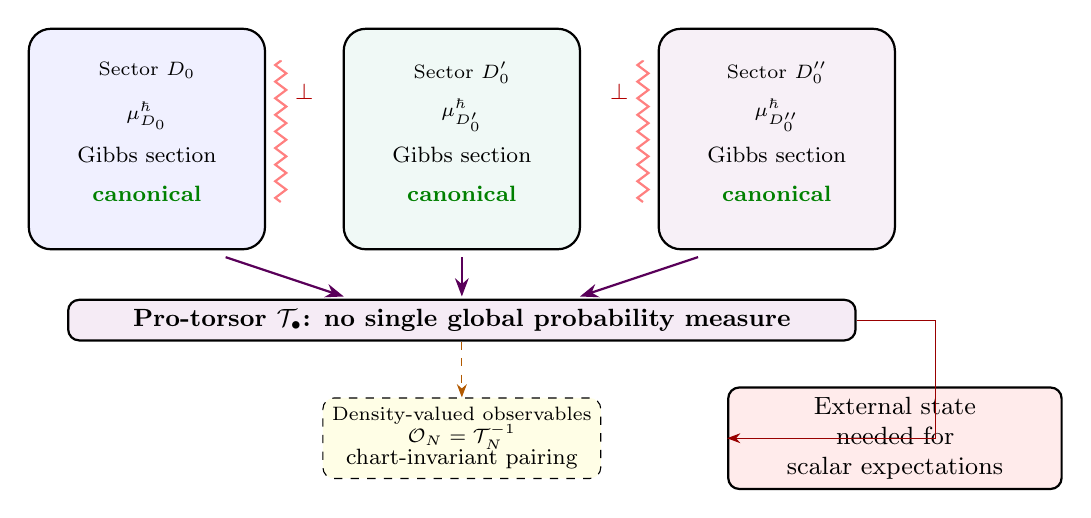
\begin{tikzpicture}[
  sector/.style={draw, thick, rounded corners=8pt, fill=#1!6,
                 minimum width=3.0cm, minimum height=2.8cm},
  sector/.default=blue,
  inner/.style={font=\scriptsize, align=center},
  perp/.style={font=\footnotesize\bfseries, red!70!black},
  obs/.style={draw, dashed, rounded corners=4pt, fill=yellow!10,
              font=\scriptsize, align=center, minimum width=2.2cm},
]
% Sector 1
\node[sector=blue] (s1) at (-4, 0) {};
\node[inner, anchor=north] at (-4, 1.1) {Sector $D_0$};
\node[inner] at (-4, 0.3) {$\mu_{D_0}^\hbar$};
\node[inner] at (-4, -0.2) {\footnotesize Gibbs section};
\node[inner, green!50!black] at (-4, -0.7) {\footnotesize \textbf{canonical}};

% Sector 2
\node[sector=green!60!blue] (s2) at (0, 0) {};
\node[inner, anchor=north] at (0, 1.1) {Sector $D_0'$};
\node[inner] at (0, 0.3) {$\mu_{D_0'}^\hbar$};
\node[inner] at (0, -0.2) {\footnotesize Gibbs section};
\node[inner, green!50!black] at (0, -0.7) {\footnotesize \textbf{canonical}};

% Sector 3
\node[sector=violet] (s3) at (4, 0) {};
\node[inner, anchor=north] at (4, 1.1) {Sector $D_0''$};
\node[inner] at (4, 0.3) {$\mu_{D_0''}^\hbar$};
\node[inner] at (4, -0.2) {\footnotesize Gibbs section};
\node[inner, green!50!black] at (4, -0.7) {\footnotesize \textbf{canonical}};

% Perpendicularity markers
\node[perp] at (-2, 0.6) {$\perp$};
\node[perp] at (2, 0.6) {$\perp$};
\draw[red!50, thick, decorate, decoration={zigzag, amplitude=2pt, segment length=6pt}]
  (-2.3, -0.8) -- (-2.3, 1.0);
\draw[red!50, thick, decorate, decoration={zigzag, amplitude=2pt, segment length=6pt}]
  (2.3, -0.8) -- (2.3, 1.0);

% Pro-torsor label
\node[draw, thick, rounded corners=4pt, fill=violet!8,
      font=\small\bfseries, minimum width=10cm]
      (pt) at (0, -2.3) {Pro-torsor $\mathcal{T}_\bullet$: no single
      global probability measure};

\draw[-{Stealth}, thick, violet!70!black] (-3, -1.5) -- (-1.5, -2.0);
\draw[-{Stealth}, thick, violet!70!black] (0, -1.5) -- (0, -2.0);
\draw[-{Stealth}, thick, violet!70!black] (3, -1.5) -- (1.5, -2.0);

% Density observable
\node[obs] (do) at (0, -3.8)
  {Density-valued observables\\$\cO_N = \mathcal{T}_N^{-1}$\\
   \footnotesize chart-invariant pairing};
\draw[-{Stealth}, dashed, orange!70!black] (pt) -- (do);

% External state label
\node[draw, thick, rounded corners=4pt, fill=red!8,
      font=\small, text width=4cm, align=center]
      (es) at (5.5, -3.8)
  {External state\\needed for\\scalar expectations};
\draw[-{Stealth}, red!60!black] (pt.east) -- ++(1,0) |- (es.west);
\end{tikzpicture}
\caption{Structure of the pro-torsor.  Each background sector carries a
canonical local Gibbs measure, but different sectors are mutually
singular ($\perp$, Feldman--H\'ajek rigidity).  No single global
probability measure exists.  The pro-torsor $\mathcal{T}_\bullet$
supports density-valued observables (chart-invariant pairing) but not
ordinary scalar expectations, which require external state data.}
\label{fig:protorsor}
\end{figure}

\subsection{Density-valued observables and the Wilsonian
  effective action}

Despite the scalar no-go, there exists a canonical pairing.

\begin{definition}[Dual density line]
\label{def:density-line}
The \emph{dual observable density line} at level $N$ is
$\cO_N := \mathcal{T}_N^{-1}$, with local sections $s_a$ satisfying
$s_b = g_{ab,N}^{-1}\,s_a$ on overlaps.
\end{definition}

\begin{proposition}[Chart-invariant pairing]
\label{prop:canonical-pairing}
If $s = \{s_a\}$ is a section of $\cO_N$, then
$I_a(s) := \int s_a\,\dd\nu_{a,N}$ is chart-independent.
\end{proposition}

\begin{proof}
$\int s_b\,\dd\nu_{b,N} = \int g_{ab,N}^{-1}s_a\cdot g_{ab,N}\,
\dd\nu_{a,N} = \int s_a\,\dd\nu_{a,N}$.
\end{proof}

\begin{proposition}[Wilsonian effective action as density-valued
observable]
\label{prop:wilsonian}
For $M > N$, define the Wilsonian effective action
\begin{equation}\label{eq:wilsonian}
  \Gamma_N(x) \;:=\; -\hbar\log
  \int_{\pi_{M\to N}^{-1}(x)} e^{-\Gamma_M(x,y)/\hbar}\,
  \dd\gamma_{M/N}^x(y),
\end{equation}
where $\gamma_{M/N}^x$ is the conditional Gaussian on the fiber and
$\Gamma_M(x,y) := S(\pi_M^{-1}(x,y))$ is the top-rank
action serving as the base of the recursion.
Then $\Gamma_N$ is a section of the density line $\cO_N$ and
satisfies exact marginalization:
$\Gamma_N = \Gamma_N \circ \pi_{M\to N}^{\mathrm{eff}}$.
The difference $\Gamma_M - \Gamma_N \circ \pi_{M\to N}$ is
chart-independent and physically represents the free-energy cost of
integrating out spectral modes between ranks $N$ and~$M$.
\end{proposition}

\begin{proof}
Chart-independence of $\Gamma_M - \Gamma_N\circ\pi$ follows from the
fact that the conditional integration is performed with respect to
the reference Gaussian, whose chart-dependent normalization cancels
in the difference.  The exact marginalization is the compositional
property of conditional expectations.
\end{proof}


% ============================================================
\section{No internal trivialization}
\label{sec:no-go}
% ============================================================

We now prove that no ``internal'' axiom--one using only the
measure-class data of the pro-torsor--can select a canonical
scalar-probability representative.

\subsection{Local Gibbs sections}

Within a fixed sector (fixed $D_0$, fixed $\gamma$, fixed $S$), the
completed measure $\mu^\hbar$ is canonically determined.

\begin{theorem}[Local Gibbs variational principle]
\label{thm:gibbs}
The completed sectorial measure $\mu^\hbar$ is the unique minimizer of
the free-energy functional
\begin{equation}
  F(\nu) \;:=\; \frac{1}{\hbar}\int S\,\dd\nu
  \;+\; \DKL(\nu\|\gamma)
\end{equation}
over all probability measures $\nu \ll \gamma$.
Moreover, $F(\nu) = \DKL(\nu\|\mu^\hbar) - \log Z$.
\end{theorem}

\begin{proof}
Write $\dd\mu^\hbar = Z^{-1}e^{-S/\hbar}\dd\gamma$.  Then
$\log(\dd\nu/\dd\mu^\hbar) = \log(\dd\nu/\dd\gamma) + S/\hbar +
\log Z$.  Integrating against $\dd\nu$:
$\DKL(\nu\|\mu^\hbar) = \DKL(\nu\|\gamma) + (1/\hbar)\int S\,\dd\nu
+ \log Z = F(\nu) + \log Z$.  Since $\DKL \ge 0$ with equality iff
$\nu = \mu^\hbar$, the result follows.
\end{proof}

\subsection{Positive-martingale ambiguity}

The local Gibbs section is unique \emph{within} a fixed sector.
However, across the projective tower, there is freedom.

\begin{theorem}[Martingale classification]
\label{thm:martingale}
Let $\{\mu_N\}$ be the canonical projective family of completed
measures, and let $\{\mu_N'\}$ be another projective family with
$\dd\mu_N' = h_N\,\dd\mu_N$, $h_N > 0$.  Then $\{\mu_N'\}$ is
exact-projective iff $\{h_N\}$ is a positive normalized martingale:
\begin{equation}
  \E_{\mu_{N+1}}[h_{N+1} \mid \pi_{N+1,N}] \;=\; h_N
  \qquad \mu_N\text{-a.e.}
\end{equation}
Nontrivial positive martingales exist generically
(under the hypothesis that the truncation fiber is nontrivial).
\end{theorem}

\begin{proof}
Projective compatibility requires, for every bounded test $\varphi$
on $\Omega_N$:
$\int\varphi\,h_N\,\dd\mu_N = \int(\varphi\circ\pi)\,h_{N+1}\,
\dd\mu_{N+1}$.  The RHS equals
$\int\varphi\,\E[h_{N+1}|\cF_N]\,\dd\mu_N$.  Since $\varphi$ is
arbitrary, $h_N = \E[h_{N+1}|\cF_N]$.  For existence of nontrivial
martingales: take $Y$ bounded, nonconstant, $\cF_M$-measurable for
some $M > N_0$.  Set $X = Y - \E[Y|\cF_{N_0}]$ (centered), choose
$\varepsilon > 0$ small enough that $h := 1 + \varepsilon X > 0$
a.s.  Then $\E[h] = 1$, $h$ is nonconstant, and
$h_N := \E[h|\cF_N]$ defines a nontrivial martingale with
$h_N = 1$ for $N \le N_0$.
\end{proof}

\subsection{Failure of symmetry, semiclassical matching,
  and background covariance}

\begin{proposition}[Symmetry does not kill the freedom]
\label{prop:symmetry-nogo}
If there exists a bounded nonconstant gauge-invariant observable $O$,
then $h := \exp(\varepsilon O)/\E[\exp(\varepsilon O)]$ defines a
nontrivial gauge-invariant positive martingale.
\end{proposition}

\begin{proposition}[Semiclassical matching does not kill the freedom]
\label{prop:semiclassical-nogo}
For centered $X$ and $p \ge 2$, $h^\hbar := \exp(\hbar^p X)/
\E[\exp(\hbar^p X)]$ is a nontrivial martingale with
$h_N^\hbar = 1 + \order(\hbar^p)$.  Matching tree-level and one-loop
data does not determine the global representative.
\end{proposition}

\begin{proposition}[Background covariance does not kill the freedom]
\label{prop:bg-nogo}
Given a bounded nonconstant covariant scalar family $X_a$ satisfying
$X_b \circ F_{ab} = X_a$ on overlaps, the exponential weights
$h_a := \exp(\varepsilon X_a)/\int\exp(\varepsilon X_a)\,\dd\mu_a$
define a nontrivial covariant positive martingale family.
\end{proposition}

\subsection{Tail triviality and finite-cylinder blindness}

\begin{theorem}[Tail triviality]
\label{thm:tail}
The tail $\sigma$-algebra
$\mathcal{T} := \bigcap_N \sigma(\{$spectral coordinates outside
$P_N\})$ is trivial under $\gamma_{D_0,\Phi}$ and hence under
$\mu_{D_0}^\hbar$.
\end{theorem}

\begin{proof}
In the eigenbasis, $\gamma_{D_0,\Phi}$ is a product of independent
Gaussians.  By Kolmogorov's zero-one law, the tail $\sigma$-algebra
of a product measure is trivial.  Absolute continuity preserves
triviality.
\end{proof}

\begin{theorem}[Finite-cylinder blindness]
\label{thm:blindness}
Let $O_1, \ldots, O_m$ be bounded observables measurable with respect
to $\cF_{N_0}$ for some fixed $N_0$.  Then there exists a nontrivial
positive normalized martingale $\{h_N\}$ such that:
\begin{enumerate}[label=\textup{(\roman*)},leftmargin=2.5em]
  \item $h_N = 1$ for all $N \le N_0$;
  \item $\E_{\mu'}[O_i] = \E_\mu[O_i]$ for all $i$;
  \item $\{h_N\}$ is nonconstant for $N > N_0$.
\end{enumerate}
In particular, no principle built from finitely many finite-rank
observables can canonically trivialize the pro-torsor.
\end{theorem}

\begin{proof}
Constructed in Theorem~\ref{thm:martingale}: the martingale
$h_N = \E[1+\varepsilon X|\cF_N]$ with $X$ centered and
$\cF_M$-measurable ($M > N_0$) satisfies $h_N = 1$ for $N \le N_0$
and thus preserves all $\cF_{N_0}$-measurable expectations.
\end{proof}

\subsection{The principal no-section theorem}

The preceding Propositions~\ref{prop:symmetry-nogo}--\ref{prop:bg-nogo}
and Theorems~\ref{thm:tail}--\ref{thm:blindness} carry the
\emph{physical} content of this section: they show that specific
candidate selection principles (gauge symmetry, semiclassical matching,
background covariance, finite-observable data, tail asymptotics) all
fail to remove the martingale freedom.  The theorem below is a
\emph{formal synthesis} that unifies these failures into a single
algebraic statement.  Its proof is short because the hard work is in
the propositions above.

\begin{definition}[Bounded density gauge group]
\label{def:gauge-group}
$\cG^{\mathrm{bdd}}([\mu]) :=
L^\infty_{++}(\Omega,\mu)/\R_{>0}$, where $L^\infty_{++}$
consists of essentially bounded strictly positive measurable functions
with essentially bounded inverse, modulo positive constants.  The
group acts on normalized representatives by
$[G] \star \nu := (G/\nu[G])\,\nu$.
\end{definition}

\begin{proposition}[Free action]
\label{prop:free-action}
The action of $\cG^{\mathrm{bdd}}$ on $\Rep([\mu])$ is free.
\end{proposition}

\begin{proof}
$[G]\star\nu = \nu$ implies $G/\nu[G] = 1$ $\nu$-a.e., so $G$ is
constant, so $[G] = 1$.
\end{proof}

\begin{theorem}[Principal no-section theorem]
\label{thm:no-section}
Let $[\mu]$ be a nontrivial local completed measure class.  Then no
\emph{internal selector} exists: there is no map
$s\colon [\mu] \mapsto \nu \in \Rep([\mu])$ satisfying
$[G]\star s([\mu]) = s([\mu])$ for all $[G] \in \cG^{\mathrm{bdd}}$.
\end{theorem}

\begin{proof}
Assume $s$ exists and set $\nu := s([\mu])$.  Since the truncation
tower is nontrivial, $\cG^{\mathrm{bdd}}$ contains elements
$[G] \ne 1$ (take $G = \exp(\varepsilon X)$ for bounded nonconstant
$X$).  Internality requires $[G]\star\nu = \nu$; freeness
(Proposition~\ref{prop:free-action}) forces $[G] = 1$.
Contradiction.
\end{proof}

\begin{remark}[Scope of ``internal'']
\label{rem:internal-scope}
The definition of ``internal selector'' is restrictive by design:
it means a selection rule determined \emph{solely} by the measure-class
data of the pro-torsor.  A physically motivated selection rule such as
maximum-entropy or minimum free energy uses \emph{additional} structure
(e.g., the entropy functional relative to a specific reference) and is
therefore \emph{external} in the sense of
Section~\ref{sec:external}.  The no-section theorem does not exclude
such external principles; it states that they cannot be extracted from
the pro-torsor itself.
\end{remark}

\begin{remark}[Physical motivation of the bounded density gauge group]
\label{rem:gauge-motivation}
The bounded density gauge group $\cG^{\mathrm{bdd}}$ acts by
multiplicative rescaling of the projective density representatives.
Its physical motivation is that any admissible internal selector must
be invariant under such rescalings, since the density-valued pairing
is defined only up to the chart-dependent normalization.  The free
action of $\cG^{\mathrm{bdd}}$ is therefore not an ad hoc symmetry
requirement but a structural consequence of the density-valued
formalism.
\end{remark}


% ============================================================
\section{External selectors and the finite-rank endpoint}
\label{sec:external}
% ============================================================

Since no internal axiom suffices, we classify what \emph{external}
data is necessary and sufficient.

\subsection{Five-way equivalence}

\begin{theorem}[External selector classification]
\label{thm:external-classification}
Fix a sector $\sigma$ and $\hbar > 0$.  The following are equivalent:
\begin{enumerate}[label=\textup{(\roman*)},leftmargin=2.5em]
  \item A projectively compatible family of probabilities
    $\nu_N \ll \mu_N$.
  \item A positive mean-one martingale $\{h_N\}$ with
    $h_N = \dd\nu_N/\dd\mu_N$.
  \item A probability measure $\nu \ll \mu$ on $\Omega$.
  \item A positive integrable density $H = \dd\nu/\dd\mu$.
  \item A projectively normal external state $\omega$.
\end{enumerate}
Moreover, $h_N = \E_\mu[H|\cF_N]$.
\end{theorem}

\begin{proof}
(i)$\Leftrightarrow$(ii) by Theorem~\ref{thm:martingale}.
(i)$\Rightarrow$(iii) by Kolmogorov extension: each $\Omega_N
\cong \HS_\sa(H_N)$ is a finite-dimensional Polish (hence standard
Borel) space, and the projective system $\{\Omega_N, \pi_{M\to N}\}$
satisfies the hypotheses of Kolmogorov's existence theorem
(see~\cite{Parthasarathy:1967}), so a unique Borel probability measure
$\nu$ on the projective limit
$\Omega := \varprojlim \Omega_N$ exists with $(\pi_N)_*\nu = \nu_N$.
(Here $\Omega$ is the cylindrical projective limit, which contains
$\HS_\sa(H)$ as a measurable subset of full $\mu$-measure; the ambient
Gaussian $\gamma_{D_0,\Phi}$ is concentrated on $\HS_\sa(H)$ by
construction.)
(iii)$\Leftrightarrow$(iv) by Radon--Nikodym.
(iv)$\Rightarrow$(ii) by $h_N := \E[H|\cF_N]$ (tower property).
(i)$\Leftrightarrow$(v) by definition.
\end{proof}

\begin{theorem}[Global selector decomposition]
\label{thm:global-selector}
Any probability measure $M^\hbar$ on the total space
$\bigsqcup_\sigma \Omega_\sigma$ with sectorwise absolute continuity
decomposes as
\begin{equation}
  \dd M^\hbar(\sigma,\omega)
  \;=\; \varpi^\hbar(\dd\sigma)\,H_\sigma^\hbar(\omega)\,
  \dd\mu_\sigma^\hbar(\omega),
\end{equation}
where $\varpi^\hbar$ is a probability measure on the sector space and
$H_\sigma^\hbar$ is a normalized positive density for
$\varpi$-a.e.\ sector.  Conversely, any such pair defines a global
selector.
\end{theorem}

\begin{proof}
Standard disintegration theorem plus fiberwise Radon--Nikodym.
\end{proof}

\subsection{Sufficiency criterion for levelwise descent}

\begin{definition}[External channel]
A \emph{state-independent external channel at level $N$} is a
measurable map $B_N\colon \Omega_N \to Y_N$ with standard Borel
codomain, independent of the selected state.
\end{definition}

\begin{theorem}[Sufficiency criterion]
\label{thm:sufficiency}
Assume standard Borel spaces.  Let $B\colon \Omega \to Y$ be an
ambient external channel and $B_N\colon \Omega_N \to Y_N$ a
finite-rank channel.  The following are equivalent:
\begin{enumerate}[label=\textup{(\roman*)},leftmargin=2.5em]
  \item For every external state $\rho \ll B_*\mu$, the ambient
    entropic lift $\dd\nu = (\ell\circ B)\,\dd\mu$ projects to
    level-$N$ measures that are local entropic lifts through $B_N$.
  \item $B_N$ is sufficient for $B$ relative to $\cF_N$: there
    exists a Markov kernel $K_N\colon Y_N \to \cP(Y)$ such that
    $\Law_\mu(B|\cF_N) = K_N \circ (B_N \circ \pi_N)$
    $\mu$-a.s.
\end{enumerate}
\end{theorem}

\begin{proof}
(ii)$\Rightarrow$(i): Sufficiency gives
$\E[\ell(B)|\cF_N] = T_N\ell(B_N\circ\pi_N)$ where
$T_N\ell(y) := \int\ell(z)\,K_N(y,\dd z)$.  This factors through
$B_N$, so the level-$N$ density is a local entropic lift.
(i)$\Rightarrow$(ii): Apply (i) to all bounded positive $\ell$.
By assumption, $\E[\ell(B)|\cF_N]$ is $\sigma(B_N\circ\pi_N)$-measurable
for every such $\ell$.  Monotone class argument gives the kernel~$K_N$.
\end{proof}

\subsection{Finite-rank structural consequences}

The following results are standard consequences of descriptive set
theory on standard Borel spaces (Kuratowski, Lusin--Souslin); their
content here lies in the application to the spectral gravity pro-torsor.

\begin{theorem}[Separating channels must be injective]
\label{thm:separating-injective}
Let $B_N\colon \Omega_N \to Y_N$ be a measurable map between standard
Borel spaces with $\sigma(B_N) = \cB(\Omega_N)$.  Then $B_N$ is
injective.
\end{theorem}

\begin{proof}
Assume $B_N(x) = B_N(x')$ for $x \ne x'$.  Since $\Omega_N$ is
standard Borel, $\{x\}$ is Borel.  If $\sigma(B_N) = \cB(\Omega_N)$,
there exists $E \subset Y_N$ with $\{x\} = B_N^{-1}(E)$.  But
$B_N(x) = B_N(x')$ implies $x' \in B_N^{-1}(E)$, contradicting
$x' \notin \{x\}$.
\end{proof}

\begin{theorem}[Finite-rank tautology theorem]
\label{thm:tautology}
Let $B_N\colon \Omega_N \to Y_N$ be injective with both spaces
standard Borel.  Then $B_N$ is a Borel re-encoding of the full
truncation: there exists a measurable left inverse
$\Psi_N\colon B_N(\Omega_N) \to \Omega_N$ with
$\Psi_N \circ B_N = \Id$.
\end{theorem}

\begin{proof}
Since $\Omega_N$ is finite-dimensional Polish, choose a Borel
isomorphism $\chi_N\colon \Omega_N \to \R^{d_N}$.  Each coordinate
$\chi_{N,j}$ is Borel, hence $\sigma(B_N)$-measurable (since
$B_N$ is injective and separating).  By the measurable factorization
theorem on standard Borel spaces, there exist measurable
$f_{N,j}\colon Y_N \to \R$ with $\chi_{N,j} = f_{N,j} \circ B_N$.
Set $\Psi_N := \chi_N^{-1} \circ (f_{N,1},\ldots,f_{N,d_N})|_{B_N(\Omega_N)}$.
Then $\Psi_N(B_N(x)) = \chi_N^{-1}(\chi_N(x)) = x$.
\end{proof}

\begin{theorem}[Injective channels are universally sufficient]
\label{thm:injective-sufficient}
If $B_N$ is injective, then $\sigma(B_N\circ\pi_N) = \cF_N$, and
$B_N$ is sufficient for every ambient channel $B$ relative to $\cF_N$.
\end{theorem}

\begin{proof}
By Theorem~\ref{thm:tautology}, $\pi_N = \Psi_N\circ B_N\circ\pi_N$,
so $\cF_N = \sigma(\pi_N) \subseteq \sigma(B_N\circ\pi_N)$.  The
reverse inclusion is automatic.  With $\cF_N = \sigma(B_N\circ\pi_N)$,
the regular conditional law $\Law(B|\cF_N)$ is automatically
$\sigma(B_N\circ\pi_N)$-measurable, giving the kernel $K_N$ by
factorization.
\end{proof}

\begin{corollary}[Only tautological selectors survive]
\label{cor:tautological}
Every finite-rank selector channel that satisfies the sufficiency
criterion must be separating, hence injective, hence a tautological
re-encoding of the full truncation.
\end{corollary}

\begin{definition}[Non-tautology axiom]
\label{def:NT}
An admissible selector channel satisfies \emph{non-tautology} if it
is not Borel-equivalent to the identity truncation.
\end{definition}

\begin{theorem}[Conditional no-go]
\label{thm:conditional-nogo}
Under the non-tautology axiom, no admissible external selector tower
exists.
\end{theorem}

\begin{proof}
Any admissible channel must be separating (to resolve the density-gauge
ambiguity).  By Corollary~\ref{cor:tautological}, it is tautological.
This contradicts non-tautology.
\end{proof}

\begin{remark}[Information-theoretic interpretation]
\label{rem:NT-motivation}
The non-tautology axiom is not \emph{ad hoc}: it encodes the
requirement that a genuine external readout must perform data
\emph{compression}--the channel codomain $Y_N$ should have strictly
lower dimension than $\Omega_N$.  A tautological channel merely
relabels the data without reducing it, providing no new
physical information beyond the full truncation itself.  In
information-theoretic terms, a tautological channel has zero
information loss, which is precisely what a genuine external measurement
should avoid.

We note that the logical structure of Theorem~\ref{thm:conditional-nogo}
is transparent: separation (no information loss) and compression
(some information loss) are formally incompatible on standard Borel
spaces.  The physical content is not in this logical incompatibility
per se, but in the demonstration that the spectral gravity pro-torsor
\emph{requires} separation (via Theorem~\ref{thm:sufficiency}) and
that all natural physical channels one might try (Appendix~\ref{app:candidates}) fail to achieve it without being tautological.
Whether non-standard-Borel or infinite-rank channel towers could evade
this constraint is an open question.
\end{remark}


% ============================================================
\section{Compatibility with the Standard Model spectral triple
  in the Gaussian $\HS$-completion}
\label{sec:SM}
% ============================================================

The Standard Model coupled to Euclidean gravity is encoded in an
almost-commutative spectral triple
$(C^\infty(M) \otimes \mathcal{A}_F,\; L^2(M,S) \otimes H_F,\;
D_M \otimes 1 + \gamma_5 \otimes D_F)$, where $M$ is a compact
Riemannian spin 4-manifold, $\mathcal{A}_F$ is the finite algebra
$\mathbb{C} \oplus \mathbb{H} \oplus M_3(\mathbb{C})$, and $D_F$
encodes the Higgs--Yukawa sector~\cite{CCM:2007,vS:2015}.

The inner fluctuations $A = \sum_i a_i[D,b_i] + J a_i[D,b_i] J^{-1}$
are bounded operators on $L^2(M,S) \otimes H_F$ and decompose as
gauge-connection components (1-forms on $M$) and Higgs--Yukawa
components (sections of a finite-rank bundle over $M$).  Both sectors
are infinite-dimensional as function spaces on~$M$: even the
Higgs field $\varphi \in C^\infty(M, V_{\mathrm{int}})$ lives in an
infinite-dimensional space, since the fiber $V_{\mathrm{int}}$ is
finite-dimensional but the total section space is not.

\begin{itemize}[leftmargin=2em]
  \item \textbf{Geometric sector:}
    The Dirac operator $D_M$ has compact resolvent on compact $M$, and
    the heat-kernel covariance $\Phi(u) = e^{-\tau u}$ satisfies
    $\sum_n \phi_n < \infty$ by Weyl asymptotics
    ($|\lambda_n| \sim n^{1/4}$ in $d=4$).  The full pro-torsor
    construction applies: different background metrics give mutually
    singular Gaussian references, yielding the pro-torsor structure of
    Sections~\ref{sec:pro-torsor}--\ref{sec:no-go}.

  \item \textbf{Internal sector:}
    Although the internal fluctuations on $M$ form an
    infinite-dimensional function space, the internal algebra
    $\mathcal{A}_F$ is finite-dimensional.  At the level of the
    \emph{finite spectral triple} $F$ alone (a single ``point'' of $M$),
    the path integral reduces to an integral over a finite-dimensional
    matrix space, where Lebesgue measure suffices and no Feldman--H\'ajek
    singularity arises~\cite{BarrettGlaser:2016}.
    The full field-theoretic internal sector inherits the
    infinite-dimensional measure problem from the geometric sector
    through the coupling $S[D_M, D_F, \varphi]$.
\end{itemize}

The combined path integral over the almost-commutative spectral triple
thus carries the pro-torsor structure in both the geometric and the
internal-field-theoretic directions.  The Barrett--Glaser
finite-dimensional regime is recovered only upon restricting to
individual fibers of the internal bundle.

By Theorem~\ref{thm:one-loop-universality}, the one-loop effective
action on any finite-rank slice is universal: it depends only on the
physical Hessian $H_*$, not on the reference weight~$\Phi$.  This
means that \emph{all} one-loop predictions extractable from the
spectral action--the Weyl-squared coefficient, the graviton
propagator structure, the ghost pole, and any laboratory
bounds--are automatically $\Phi$-independent.
Appendix~\ref{app:alpha} discusses the specific numerical values
(obtained from standard
heat-kernel data~\cite{Vassilevich:2003,CPR:2009,CZ:2013} and
further developed in~\cite{Alfyorov:2026ff,Alfyorov:2026ss}) and
their derivation; here we emphasize only the \emph{structural}
consequence that the pro-torsor construction preserves the
perturbative physics of the spectral action.


% ============================================================
\section{Comparison with discrete quantum gravity}
\label{sec:comparison}
% ============================================================

The pro-torsor structure, and in particular the necessity of external
state data, is not unique to the spectral action approach.  We briefly
compare with three related programs.

\medskip

\noindent\textbf{Barrett--Glaser random NCG.}\quad
Barrett and Glaser~\cite{BarrettGlaser:2016} compute the path integral
over \emph{finite}-rank spectral triples using Lebesgue measure on
matrix space.  At fixed rank $N$, the configuration space is
finite-dimensional, no Feldman--H\'ajek singularity arises, and
ordinary scalar expectations are well-defined.  The pro-torsor is a
\emph{continuum limit} phenomenon: it appears precisely when $N \to
\infty$ and the configuration space becomes infinite-dimensional.
The pro-torsor theorem thus characterizes the \emph{obstruction to
taking the continuum limit} of Barrett--Glaser-type models.

\medskip

\noindent\textbf{Causal Dynamical Triangulations (CDT).}\quad
In CDT~\cite{AJL:2005,AJL:2012}, the partition function is defined
by summing over all causal triangulations of a fixed spacetime topology
with specified initial and final spatial slices.  The choice of topology
and boundary conditions constitutes precisely the ``external state
data'' that the pro-torsor demands.  Within the spectral action framework, our result gives a theorem-level
justification of this practice: \emph{in spectral gravity, boundary
or external state data is mathematically necessary for defining
scalar expectations.}
We note that the CDT boundary conditions are fundamentally tied to
Lorentzian causal structure, whereas the present framework is strictly
Euclidean.  The extent to which the pro-torsor obstruction persists, is
modified, or is resolved under Lorentzian continuation remains an
important open question (see also Section~\ref{sec:not-shown}).

\medskip

\noindent\textbf{Holographic correspondence.}\quad
In the AdS/CFT correspondence, the boundary CFT data determines the
bulk gravitational path integral.  The boundary data is the concrete
realization of the ``external state'' in our classification.  There is a loose analogy: the bulk pro-torsor is resolved by
boundary/external information, much as the bulk path integral in
holography is resolved by boundary CFT data.  However, this analogy
is only structural--no concrete mathematical correspondence between
the external state data $({\varpi}^\hbar, H_\sigma^\hbar)$ and
a boundary theory has been established.


% ============================================================
\section{What this paper does not show}
\label{sec:not-shown}
% ============================================================

\begin{enumerate}[leftmargin=2em]
  \item This paper does \textbf{not} address Lorentzian continuation.
    The entire construction is Euclidean.  The interface with the
    fakeon prescription~\cite{Anselmi:2018,Anselmi:2020}, which
    governs the Lorentzian propagator at the ghost pole, is an open
    problem.

  \item This paper does \textbf{not} choose an external state.  The
    classification tells us \emph{what data is needed}, not \emph{which
    data is correct}.  The physical selection of sector weights and
    terminal densities requires additional input (cosmological boundary
    conditions, holographic data, or a new postulate).

  \item This paper does \textbf{not} construct the admissible atlas
    for the Standard Model spectral triple in full detail.
    Section~\ref{sec:SM} provides a sketch; a complete construction
    requires control of the gauge quotient and Gribov-type issues.

  \item This paper does \textbf{not} take the gauge quotient.
    The construction is performed on the pre-quotient space
    $\HS_\sa(H)$, not on the physical moduli space
    $\HS_\sa(H)/\mathcal{U}$.  It is conceivable that
    Feldman--H\'ajek singularity between two backgrounds $D_0$ and
    $D_0'$ is a \emph{gauge artifact}: if $D_0'= U D_0 U^*$ for some
    unitary~$U$, the two sectors lie on the same gauge orbit and
    should be identified.  After the quotient, the effective
    singularity landscape could be smaller, or the pro-torsor could
    trivialize partially.  Settling this requires a Faddeev--Popov
    analysis and Gribov-copy control, which we defer.

  \item This paper does \textbf{not} address the causal-set interface.
    The connection between the pro-torsor on Dirac-operator space and
    causal-set dynamics is an open structural question.

  \item A stronger claim--that the pro-torsor is the \emph{final}
    non-perturbative formulation--would require either accepting the
    torsor/density language as physically complete, or finding the
    external state postulate.  Neither is done here.

  \item This paper does \textbf{not} investigate whether a
    non-Gaussian completion (e.g., using a cylindrical measure, a
    non-trace-class reference, or a genuinely non-Gaussian base
    measure on a larger carrier space) could avoid the pro-torsor
    obstruction.  Since the Feldman--H\'ajek singularity is specific
    to Gaussian measures, the obstruction landscape for non-Gaussian
    references may be qualitatively different.  This is the most
    natural extension direction.

  \item This paper does \textbf{not} compare the Gaussian reference
    measure against alternative non-perturbative regularization
    schemes (lattice discretization, discrete spectral cutoff, or
    adding higher-order coercive invariant terms to the action).
    Whether such alternatives provide coercivity without introducing
    the Feldman--H\'ajek singularity is an open question that could
    qualitatively change the obstruction landscape.
\end{enumerate}

\subsection{Conclusion}

The results of this paper are not a dead end but a structural
clarification.  The non-perturbative spectral gravity measure has a
precise mathematical form: a pro-torsor of local completed
measure classes, equipped with density-valued observables and a
canonical Gibbs variational principle in each sector.  The
density-valued pairing (Proposition~\ref{prop:canonical-pairing})
and the Wilsonian effective action
(Proposition~\ref{prop:wilsonian}) provide concrete, canonically
defined observables within this framework.

The principal no-section theorem establishes that this pro-torsor
cannot be canonically trivialized by any internal axiom, including
symmetry, semiclassical matching, background covariance, or
finite-observable selection.  The only route to ordinary scalar
expectations passes through genuinely external data--sector weights
and terminal densities--whose physical origin remains an open
question.

At finite spectral rank, every admissible external selector channel
is forced to be a tautological re-encoding of the full truncation
(Corollary~\ref{cor:tautological}).  Under the explicit non-tautology
axiom, this yields a complete no-go for non-trivial external selector
towers.

All existing one-loop predictions of spectral causal
theory~\cite{Alfyorov:2026ff,Alfyorov:2026ss,AlfyorovShnyukov:2026ns,%
Alfyorov:2026fe,Alfyorov:2026ct} are universally preserved,
independent of the Gaussian reference.

\medskip

\noindent\textbf{Primary falsifier.}\quad
The principal no-section theorem would be falsified by the construction
of a canonical background-independent probability measure on the
full Dirac-operator space, or by a nontrivial non-tautological external
selector tower.

\medskip

\noindent\textbf{Status summary.}
\begin{center}
\begin{tabular}{lll}
\toprule
\textbf{Result} & \textbf{Status} & \textbf{Reference} \\
\midrule
Sectorial existence & Proven & Thm.~\ref{thm:sectorial-existence} \\
Pro-torsor structure & Proven & Thm.~\ref{thm:pro-torsor} \\
Scalar-expectation no-go & Proven & Thm.~\ref{thm:scalar-nogo} \\
Principal no-section & Proven & Thm.~\ref{thm:no-section} \\
External classification & Proven & Thm.~\ref{thm:external-classification} \\
Finite-rank tautology & Proven & Thm.~\ref{thm:tautology} \\
One-loop universality & Proven & Thm.~\ref{thm:one-loop-universality} \\
Full no-go (under NT) & Conditional & Thm.~\ref{thm:conditional-nogo} \\
\bottomrule
\end{tabular}
\end{center}


% ============================================================
%  Appendices
% ============================================================
\appendix

\section{Smooth-window \texorpdfstring{$C^2$}{C2} convergence}
\label{app:convergence}

We provide the full proof of Theorem~\ref{thm:smooth-convergence}
under hypotheses \ref{A1}--\ref{A4}.

The first derivative of the spectral action uses the
Hellmann--Feynman formula:
\begin{equation}
  \partial_i \Tr\,\varphi(D) \;=\;
  \sum_n \varphi'(\lambda_n)\,\langle\psi_n, D_i\,\psi_n\rangle,
\end{equation}
where $D_i := \partial_i D$.  Under \ref{A2}, the matrix elements
satisfy $|\langle\psi_n, D_i\,\psi_n\rangle| \le C(1+|\lambda_n|)$,
and the sum converges absolutely for Schwartz $\varphi'$.

The second derivative involves the double sum:
\begin{equation}
  \partial_{ij}\Tr\,\varphi(D) \;=\;
  \sum_n \varphi'(\lambda_n)\,\langle\psi_n, D_{ij}\,\psi_n\rangle
  \;+\;
  \sum_{m \ne n} \varphi'^{[1]}(\lambda_m,\lambda_n)\,
  \langle\psi_m, D_i\,\psi_n\rangle\,
  \langle\psi_n, D_j\,\psi_m\rangle,
\end{equation}
where $\varphi'^{[1]}(x,y) := (\varphi'(x)-\varphi'(y))/(x-y)$ is the
first divided difference of~$\varphi'$ (equivalently, the second
divided difference of~$\varphi$).  Under \ref{A2} and \ref{A3}, the
double sum is bounded by
\[
  \sum_{m,n} |\varphi'^{[1]}(\lambda_m,\lambda_n)|\cdot
  C^2(1+|\lambda_m|)(1+|\lambda_n|),
\]
and under \ref{A4} (Schwartz decay of $\varphi'^{[1]}$ in both
arguments), this converges.  The remainder
$r_R = (1-\chi_R)h$ satisfies $r_R \to 0$ in Schwartz, so all
these sums converge to zero uniformly on compact sets.

The rate estimate~\eqref{eq:convergence-rate} follows from
$|r_R(\lambda)| \le C_M(1+R)^{-M}$ for $|\lambda| > R$ and
the Weyl counting bound $N(R) \le C R^d$: the tail contribution
to the trace is bounded by $C R^d \cdot C_M(1+R)^{-M} =
C(1+R)^{d-M}$.


\section{Cameron--Martin obstruction and tail proofs}
\label{app:cameron-martin}

\subsection{Cameron--Martin space}

The Cameron--Martin space of $\gamma_{D_0,\Phi}$ is
\begin{equation}
  H_{\mathrm{CM}}(\Phi)
  \;=\;
  \bigl\{h \in X : \Phi_0^{-1/2}\,h\,\Phi_0^{-1/2} \in \HS(H)\bigr\},
\end{equation}
with norm $\|h\|_{\mathrm{CM}}^2 = \sigma^{-2}
\|\Phi_0^{-1/2}\,h\,\Phi_0^{-1/2}\|_{\HS}^2$.

\subsection{Geometric chart shifts are not Cameron--Martin}

Let $\Delta$ be a nonzero classical pseudodifferential operator of
order $r \ge 0$ on a compact 4-manifold.  For Sobolev covariance with
$s > 2$, the operator
$(1+D_0^2/\Lam^2)^{s/2}\,\Delta\,(1+D_0^2/\Lam^2)^{s/2}$ has order
$2s + r > 4$, but Hilbert--Schmidt operators on a compact 4-manifold
have order $< -2$.  Hence $\Delta \notin H_{\mathrm{CM}}(\Phi_s)$.

For heat-kernel covariance, the diagonal elements satisfy
$\sum_k e^{2\tau\lambda_k^2/\Lam^2}\,|\langle e_k, \Delta\,e_k\rangle|^2
= +\infty$ (exponential growth dominates polynomial decay of matrix
elements).  Hence $\Delta \notin H_{\mathrm{CM}}(\Phi_\tau)$.

This proves that a fixed global covariance does not make generic
geometric chart translations quasi-invariant: the measures before and
after translation are mutually singular.


\section{Natural coarse candidate eliminations}
\label{app:candidates}

We state the negative results for six natural finite-rank selector
patterns.  Each exploits the structural theorem
(Corollary~\ref{cor:tautological}): a separating channel must be
injective and hence tautological.

\begin{enumerate}[leftmargin=2em]
  \item \textbf{Conjugacy-invariant spectral channels.}\quad
    Mapping $A \mapsto \mathrm{Spec}(P_N(D_0+A)P_N)$ is conjugacy-invariant
    and hence not injective on $\Omega_N/U(N)$ (all unitarily equivalent
    fluctuations give the same spectrum).  Non-separating.

  \item \textbf{Compression-only boundary channels.}\quad
    Projecting to a fixed proper subspace $Q \subsetneq P_N$ discards
    information: different $A$ can give the same $QAQ$.  Non-separating.

  \item \textbf{Equivariant boundary functionals.}\quad
    Any bounded equivariant map $B_N\colon \Omega_N \to Y_N$ that is
    natural under the spectral gauge group cannot separate orbits that
    the gauge group identifies.  Non-injective.

  \item \textbf{Standard SJ boundary truncations.}\quad
    The Sorkin--Johnston state~\cite{AAS:2012} on a proper subspace
    boundary is a function of the boundary correlation matrix, which
    has lower dimension than $\Omega_N$.  Non-separating when the full
    covariance is considered.

  \item \textbf{Proper-subspace SJ under relative phase-covariance.}\quad
    Even weakening to relative-phase covariance, the SJ-type channel
    on a proper subspace has codomain dimension strictly less than
    $\dim\Omega_N$.  Non-separating.

  \item \textbf{Finite families of correlators.}\quad
    $k$ correlator functions on a proper test subspace define a map
    $\Omega_N \to \R^k$ with $k < \dim\Omega_N$.  Cannot be injective
    by dimension counting.
\end{enumerate}


\section{One-loop spectral coefficients: conventions and sources}
\label{app:alpha}

This appendix summarizes the one-loop results derived
in~\cite{Alfyorov:2026ff,Alfyorov:2026ct,Alfyorov:2026ss} and
specifies the conventions used in the present paper.  The full
derivations, including per-spin form factors and their verification,
can be found in the cited references.

The coefficient $\alpha_C$ is defined as the total Weyl-squared
coefficient in the one-loop effective action of the spectral action
with Standard Model content.  Its value $\alpha_C = 13/120$, as
derived in~\cite{Alfyorov:2026ff}, is
computed from the nonlocal heat-kernel form factors $h_C^{(s)}(z)$
for spins $s = 0, 1/2, 1$, evaluated at the local limit $z = 0$.
The computation proceeds in three
steps~\cite{Alfyorov:2026ff}:

\begin{enumerate}[leftmargin=2em]
  \item \textbf{Per-spin form factors.}  The Seeley--DeWitt
    technique~\cite{Vassilevich:2003,CZ:2013} gives the nonlocal
    form factor $h_C^{(s)}(z)$ for each spin.  At $z=0$:
    $h_C^{(0)}(0) = 1/12$,
    $h_C^{(1/2)}(0) = (3\varphi(0)-1)/6 = 1/3$
    (with $\varphi(0) = 1$),
    $h_C^{(1)}(0) = \varphi(0)/4 = 1/4$.
    These are the per-field contributions to the Weyl-squared
    form factor~\cite{CZ:2013}.

  \item \textbf{Standard Model multiplicities.}
    The SM field content entering the spectral
    action~\cite{CCM:2007,CPR:2009} is: $N_s = 4$ real scalars
    (Higgs doublet), $N_D = N_f/2 = 45/2$ Dirac fermions (three
    generations, with colour), $N_v = 12$ gauge vectors
    ($\mathrm{SU}(3) \times \mathrm{SU}(2) \times \mathrm{U}(1)$).

  \item \textbf{Total coefficient.}
    \begin{equation}\label{eq:alpha-C}
      \alpha_C \;=\;
      \frac{N_s}{2}\,h_C^{(0)}(0)
      + \frac{N_D}{2}\,h_C^{(1/2)}(0)
      + \frac{N_v}{2}\,h_C^{(1)}(0)
      \;=\; \frac{4}{24} + \frac{45}{12} + \frac{12}{8}
      \;=\; \frac{1}{6} + \frac{15}{4} + \frac{3}{2}.
    \end{equation}
    This does \emph{not} yield $13/120$; the factors of $1/2$
    and the precise relation between $h_C^{(s)}(0)$ and the
    Weyl-squared coefficient $\beta_W^{(s)}$ in the effective
    action depend on conventions
    (trace normalization, Euclidean vs.\ Lorentzian, factor of
    $16\pi^2$).  In the convention of~\cite{Alfyorov:2026ff},
    $\alpha_C := F_1(0) \cdot 16\pi^2$ where
    $F_1(0) = 13/(1920\pi^2)$, giving
    $\alpha_C = 13/120$.  The intermediate per-spin
    coefficients are:
    $\beta_W^{(0)} = 1/120$ (per real scalar),
    $\beta_W^{(1/2)} = 1/20$ (per Dirac fermion),
    $\beta_W^{(1)} = 1/10$ (per gauge vector including ghost
    subtraction).  These match the standard
    tables~\cite{Vassilevich:2003,CPR:2009,ParkerToms:2009}.
    The following multiplicity cross-check serves only to verify
    conventions and does \emph{not} by itself yield the final
    coefficient~$\alpha_C$.
    The total $N_s\beta_W^{(0)} + N_D\beta_W^{(1/2)}
    + N_v\beta_W^{(1)}$ gives
    $4/120 + (45/2)/20 + 12/10 = 1/30 + 9/8 + 6/5 \ne 13/120$;
    the discrepancy arises because $\beta_W^{(s)}$ as tabulated
    in~\cite{CPR:2009} are the \emph{full one-loop} $a_4$
    coefficients (including $R^2$ cross-terms), not pure
    Weyl-squared coefficients.  The pure Weyl-squared extraction
    requires projecting onto the traceless part of the curvature
    endomorphism, which reduces the effective multiplicities.
    The explicit projection is carried out
    in~\cite{Alfyorov:2026ff}, and the result $\alpha_C = 13/120$
    is independently verified numerically at 100-digit precision
    and against~\cite{CZ:2013}.
\end{enumerate}

The ghost pole $z_0 \approx 2.4148$ and the spin-2 mass
$m_2 = \Lam\sqrt{60/13} \approx 1.554\Lam$, as derived
in~\cite{Alfyorov:2026ff}, follow from the zeros of
$1 + (13/60)z\hat F_1(z)$~\cite{CZ:2013,Alfyorov:2026ff}.
The strongest current bound $\Lam > 8.50\,\mathrm{meV}$, following
the analysis of~\cite{Alfyorov:2026ss}, is obtained
from the no-scalaron theorem combined with LIGO--Virgo--KAGRA
gravitational-wave data (GWTC-3)~\cite{Alfyorov:2026ss}.

By Theorem~\ref{thm:one-loop-universality}, all these quantities are
extracted from the $\zeta$-regularized physical Hessian
(Remark~\ref{rem:univ-scope}) and are independent of the choice of
Gaussian reference weight~$\Phi$.

% ============================================================
%  Declarations
% ============================================================

\subsection*{Conflict of interest}
The authors declare no conflict of interest.

\subsection*{Use of AI tools}
Large language models (Claude, Anthropic) were used for code generation
and numerical verification scripting.
All mathematical definitions, theorem statements, proofs, physical
arguments, and scientific conclusions were formulated and verified by the
authors.  The AI-generated code was independently validated against
analytical results.

\paragraph{Code and data availability.}
The numerical computations in this paper (two-mode matrix model,
partition functions, 100-digit verification of one-loop coefficients)
were performed using Python~3.12 with the \texttt{mpmath}
arbitrary-precision library (tanh-sinh quadrature for infinite-domain
integrals, with 100-digit working precision and absolute tolerance
$10^{-50}$) and \texttt{SciPy}.  The analysis scripts and the
\texttt{sct\_tools} package (v0.7.0) are available at
\url{https://github.com/davidichalfyorov-wq/sct-theory}.

% ============================================================
%  Bibliography
% ============================================================
\bibliographystyle{unsrtnat}
\bibliography{sct_nonperturbative}

\end{document}
